%----------------------------------------------------------------------------------------
%	PREAMBLE
%----------------------------------------------------------------------------------------
\documentclass[12pt]{article} % Default font size is 12pt, it can be changed here

\usepackage{geometry} % Required to change the page size to A4
\geometry{a4paper} % Set the page size to be A4 as opposed to the default US Letter
% \geometry{top=8em}
\geometry{top=8em,bottom=8em}

\usepackage{verbatim}


\def\checkmark{\tikz\fill[scale=0.4](0,.35) -- (.25,0) -- (1,.7) -- (.25,.15) -- cycle;}

\usepackage[table]{xcolor}% http://ctan.org/pkg/xcolor
\definecolor{cadmiumgreen}{rgb}{0.0, 0.42, 0.24}

\usepackage{commath}

\usepackage{etoolbox}
\usepackage{ifthen}

\usepackage{hyperref}
\hypersetup{
    colorlinks=true,
    linkcolor=black,
    filecolor=magenta,      
    urlcolor=blue,
    pdftitle={ESDPP Prelim}
} % Hyperlinks
\urlstyle{same}

\usepackage{sidecap}

\usepackage{fancyhdr}

\usepackage{gensymb}

\usepackage{graphicx} % Required for including pictures

\usepackage{array}

\usepackage{caption}

\usepackage{float} % Allows putting an [H] in \begin{figure} to specify the exact location of the figure
\usepackage{wrapfig} % Allows in-line images such as the example fish picture

\usepackage{lipsum} % Used for inserting dummy 'Lorem ipsum' text into the template - \lipsum[#]

\usepackage{amsmath,amssymb,latexsym} % Maths and maths symbols.

\usepackage{xparse}

%peter added these %%

%%

\linespread{1.2} % Line spacing

\setlength{\parindent}{0pt}

\usepackage{setspace}
\usepackage{pgfplots}
\pgfplotsset{every axis/.append style={
    font=\footnotesize,
    thin,
    tick style={thin}}}
\usetikzlibrary{patterns}
\usepgflibrary{patterns}
\pgfplotsset{compat=1.5.1}
% \usepackage{circuitikz}
\usetikzlibrary{decorations.markings}
\usetikzlibrary{calc,intersections}
\usetikzlibrary{positioning}
\usetikzlibrary{arrows, arrows.meta, decorations.pathmorphing, decorations, shapes}
\usepackage{cancel}

\tikzset{
    position label/.style={
       below = 3pt,
       text height = 1.5ex,
       text depth = 1ex
    },
   brace/.style={
     decoration={brace, mirror},
     decorate
   }
}



%\setlength\parindent{0pt} % Uncomment to remove all indentation from paragraphs

\graphicspath{{Pictures/}} % Specifies the directory where pictures are stored

%Table%
\usepackage{array}
\newcolumntype{L}[1]{>{\raggedright\let\newline\\\arraybackslash\hspace{0pt}}m{#1}}
\newcolumntype{C}[1]{>{\centering\let\newline\\\arraybackslash\hspace{0pt}}m{#1}}
\newcolumntype{R}[1]{>{\raggedleft\let\newline\\\arraybackslash\hspace{0pt}}m{#1}}

\newcommand{\note}[2]{{\color{red}{[#1] #2}}}


\usepackage{listings}
\usepackage{xcolor}

%New colors defined below
\definecolor{codegreen}{rgb}{0,0.6,0}
\definecolor{codegray}{rgb}{0.5,0.5,0.5}
\definecolor{codepurple}{rgb}{0.58,0,0.82}
\definecolor{backcolour}{rgb}{0.95,0.95,0.92}

%Code listing style named "mystyle"
\lstdefinestyle{mystyle}{
%   backgroundcolor=\color{backcolour},
  commentstyle=\color{codegreen},
  keywordstyle=\color{magenta},
  numberstyle=\tiny\color{codegray},
  stringstyle=\color{codepurple},
  basicstyle=\ttfamily\footnotesize,
  breakatwhitespace=false,         
  breaklines=true,                 
  captionpos=b,                    
  keepspaces=true,                 
  numbers=left,                    
  numbersep=5pt,                  
  showspaces=false,                
  showstringspaces=false,
  showtabs=false,                  
  tabsize=2,
  frame=tblr,
}

%"mystyle" code listing set
\lstset{style=mystyle}


\renewcommand{\lstlistlistingname}{List of Listings}
\usepackage[title]{appendix}
\usepackage{pdfpages}
\usepackage{amsmath}
\usepackage{enumitem}
\usepackage{amssymb}
\usepackage{wasysym}
\usepackage{graphicx}
\usepackage{geometry}

\usepackage{import}

\usepackage{cleveref}


\usepackage{makecell}
\usepackage{xspace}
\usepackage{multicol}
\usepackage{multirow}
\usepackage{tikz}
\usetikzlibrary{patterns,arrows}
\usepackage[english]{babel}
\usepackage{appendix}
\usepackage{pdflscape}
\usepackage{caption}
\usepackage{subcaption}
\usepackage{rotating}
\linespread{1.2} %line spacing
\newcommand{\HRule}{\rule{\linewidth}{0.5mm}}
\usepackage[T1]{fontenc}
\usepackage{bigfoot} % to allow verbatim in footnote
\usepackage[numbered,framed]{matlab-prettifier}
\usepackage{filecontents}
\usepackage[document]{ragged2e}
\usepackage{float}
\usepackage{natbib}
\usepackage{longtable} % double page table
\usepackage{multirow}
\usepackage{blindtext}
% \usepackage{longtable}

%table packages
\usepackage{rotating}
\usepackage{adjustbox}
\usepackage[table]{xcolor}

\hypersetup{%
   citecolor=black
}

\usepackage{tikz}
\newcommand\diag[4]{%
  \multicolumn{1}{p{#2}|}{\hskip-\tabcolsep
  $\vcenter{\begin{tikzpicture}[baseline=0,anchor=south west,inner sep=#1]
  \path[use as bounding box] (0,0) rectangle (#2+2\tabcolsep,\baselineskip);
  \node[minimum width={#2+2\tabcolsep-\pgflinewidth},
        minimum  height=\baselineskip+\extrarowheight-\pgflinewidth] (box) {};
  \draw[line cap=round] (box.north west) -- (box.south east);
  \node[anchor=south west] at (box.south west) {#3};
  \node[anchor=north east] at (box.north east) {#4};
 \end{tikzpicture}}$\hskip-\tabcolsep}}

\begin{document}


%%%%%%%%%%%%%%%%%%%%%%%%%%%%%
%	TITLE PAGE DEFINITION
%%%%%%%%%%%%%%%%%%%%%%%%%%%%%

\newcommand*{\titleGP}{\begingroup % Create the command for including the title page in the document
\centering % Center all text
%\vspace*{\baselineskip} % White space at the top of the page

\rule{\textwidth}{1.2pt}\vspace*{-\baselineskip}\vspace*{2pt} % Thick horizontal line
\rule{\textwidth}{0.4pt}\\[\baselineskip] % Thin horizontal line

{\LARGE \textsc{ASRA}\\[0.3\baselineskip]
\Large \textsc{Aerial Surveillance Response Aircraft}\\[0.3\baselineskip]
\textsc{Preliminatry Report}}\\[0.2\baselineskip] % Title
\note{Rhys}{Include Honours number}

\rule{\textwidth}{0.4pt}\vspace*{-\baselineskip}\vspace{3.2pt} % Thin horizontal line
\rule{\textwidth}{1.2pt}\\[\baselineskip] % Thick horizontal line

\scshape % Small caps
% Creating a CLTF for a IVHS whilst satisfying numerous design constraints.\\[0.3\baselineskip] % Tagline(s) or further description
{\scshape\today} \\ % Date published

\vspace*{3.5\baselineskip} % Whitespace between location/year and editors

Written by \\[0.3\baselineskip]
{\Large Peter Conway, a1703723\par} % Editor list
{\Large Samuel Drown, a1716243\par} % Editor list
{\Large Harry Lukasz, a1721127\par} % Editor list
{\Large Thomas Walker, a1705672\par} % Editor list
{\Large Jake Williams, a1717794\par} % Editor list
{\Large Rhys Wilson, a1725922\par} % Editor list



%\vspace*{6cm} % White space at the top of the page

\vfill

\includegraphics[width=.3\textwidth]{Figures/logo.pdf}\\


\endgroup}

%%%%%%%%%%%%%%%%%%%%%%%%%%%%%
%	TITLE PAGE
%%%%%%%%%%%%%%%%%%%%%%%%%%%%%

\pagestyle{empty}

\titleGP % This command includes the title page

\newpage


%%%%%%%%%%%%%%%%%%%%%%%%%%%%%
%	TITLE PAGE
%%%%%%%%%%%%%%%%%%%%%%%%%%%%%

\newpage

\pagenumbering{roman}
\setcounter{page}{1}

\pagestyle{fancy}
\fancyhf{}
\fancyhead[C]{Preliminary Report}

\fancyfoot[C]{\thepage}

\newpage
%\phantom{.}
%\thispagestyle{empty}
%
%\newpage
%\setcounter{page}{2}


\section*{Acknowledgements}
\addcontentsline{toc}{section}{\protect\hphantom{\numberline{\thesection}}Acknowledgements}

% Not sure if people want this

We would like to thank the following organisations and individuals for their contribution to and support of the project thus far.

\begin{itemize}
    \item The University of Adelaide:
    \begin{itemize}
        \item Dr Rey Chin
    \end{itemize}
    \item Lockheed Martin STELaRLab:
    \begin{itemize}
        \item Dr Tim Payne
        \item Dr Scott Beinke
    \end{itemize}
 
\end{itemize}

%%%%%%%%%%%%%%%%%%%%%%%%%%%%%
\vspace{2cm}
\newpage
\section*{Glossary}
\addcontentsline{toc}{section}{\protect\hphantom{\numberline{\thesection}}Glossary}

Table \ref{tab:definitions} defines acronyms and technical jargon used throughout the following document. 

\begin{table}[h!]
    \centering
    \caption{Glossary of Terms}
    \label{tab:definitions}
    \begin{tabular}{l|l}
        Concept & Definition\\\hline
        Airframe & The body of an aircraft as distinct from its engine\\
        CAD & Computer Aided Design\\
        CASA & Civil Aviation Safety Authority\\
        CFD & Computational Fluid Dynamics\\
        CFS & Country Fire Service\\
        COTS & Component of the Shelf\\
        FPV & First Person View\\
        RPA & Remotely Piloted Aircraft\\
        UAV & Unmanned Aerial Vehicle \\
        URAF & Unmanned Research Aircraft Facility\\
        UART & Universal Asynchronous Receiver Transmitter\\
        VTOL & Vertical Take Off and Landing\\
        eVTOL & electric Vertical Take Off and Landing\\
        ICE & Internal Composition Engine\\
        BLDC & Brushless Direct Current\\
        Li-po & Lithium Polymer\\
        ESC & Electric Speed Controller\\
        FC & Flight Controller\\
    \end{tabular}
\end{table}

\section*{Nomenclature}
\begin{minipage}{.5\textwidth}
\noindent\begin{longtable*}{@{}l @{\quad=\quad} l@{} @{}l @{\quad=\quad} l@{}}
$M$  & Mass \\
$W$  & Weight \\
$MF$   & Mass Fraction \\
$P$ & Power \\
$T$ & Thrust \\
$L$ & Lift \\
$D$ & Drag \\
$C_l$ & Lift Coefficient \\
$C_d$ & Drag Coefficient \\
$PL$ & Power Loading \\
$S$ & Wing Area \\
$WS$ & Wing Loading \\
$A$ & Disk Area \\
$\rho$ & Air Density \\
$AR$ & Aspect Ratio \\
$e_o$ & Oswald efficiency factor\\
$e_{batt}$ & Battery Specific Energy\\

\end{longtable*}%}
\end{minipage}
\begin{minipage}{.5\textwidth}
\noindent\begin{longtable*}{@{}l @{\quad=\quad} l@{} @{}l @{\quad=\quad} l@{}}
$E$ & Energy \\
$q$ & Dynamic Pressure \\
$RC$ & Rate if Climb \\
$\eta$ & Efficiency\\
$F$ & Fraction\\
$SF$ & Safety Factor\\
$t$ & time \\
$v$ & velocity \\
\end{longtable*}%}
$Subscripts$  \\
\noindent\begin{longtable*}{@{}l @{\quad=\quad} l@{} @{}l @{\quad=\quad} l@{}}
$batt$ & battery \\
$PL$ & payload \\
$TOW$ & Take-off Weight \\
$Req$ & Required \\
$max$ & Maximum \\
$i$ & Segment \\
$\infty$ & Free Stream \\
\end{longtable*}%}
\end{minipage}


\newpage
%\phantom{.}
%\thispagestyle{empty}
%
%\newpage
%\setcounter{page}{3}

\justifying
\section*{Executive Summary}
\addcontentsline{toc}{section}{\protect\hphantom{\numberline{\thesection}}Executive Summary}

This report presents the preliminary design and analysis for a long range, Vertical Take Off and Landing (VTOL), Unmanned Aerial Vehicle (UAV). Through discussion with the Country Fire Service (CFS) the need for a VTOL UAV, to conduct bushfire scar scanning was identified. A detailed set of project objectives was developed from these discussions, through which specific system requirements were identified and a worse case mission profile developed. Based on quantitative analysis and understanding of fundamental aerodynamic principals these designs were ranked according to how well they fulfilled the project objectives. Two subsequent rounds of concept generation were undertaken culminating in two designs which were extensively evaluated through conducting preliminary sizing and determining required power consumption for completion of the worst case mission profile. From this a design was identified with a required battery weight of 3.185 kg. The final design is based upon a canard configuration which utilises a tilt-wing mechanism and modular wings to allow for continuing analysis in optimum propulsion system. The tilt-wing mechanism is designed to achieve an angular wing rotation of approximately 140 degrees and capacity to withstand 2.51 Nm of torque. The selected camera payload system was the FireFlight 3000, comprised of 2 Infra-Red (IR) Cameras and a Red Green Blue (RGB) camera, which performs on board monitoring and analysis of the bushfire area. At the allowable operating height of 400ft, stipulated by CASA regulations, this payload provides a spatial resolution of {0.2m$^2$}, sufficient for the monitoring applications identified. A prototype has been developed to ascertain the control complexities of the proposed device. The selected Programmable Flight controller for a low end prototype system is the Matek Systems F405-STD. This flight controller will integrate with preliminary power electronics to form a minimum complexity VTOL system to explore control feasibility. A preliminary system was developed for the computer vision landing site detection using sample images with proven success. \\

High level risk analysis reveled the potential that stakeholder expectations of innovation may not be met, due to tight timelines imposed on the design and research stages as a result of meeting workshop manufacturing deadlines. To adhere to requirements of both industrial and academic stakeholders, two desired project outcomes were identified. A Minimal Viable Product (MVP) containing elements of the systems described above, will be manufactured following a simple prototype stage intended to confirm projected aircraft control capabilities. The MVP is necessary for physical testing and validation of the design analysis and methodology thus satisfying academic requirements. In parallel, continued research will be conducted in optimising the overall design and investigating opportunities to improve flight efficiencies, fulfilling industrial requirements. Provided the MVP verifies the theoretical analysis, increased confidence may be placed on the optimised design, with increased complexity, to perform as expected. Project management projections expect the project to conclude within the required time frame, and within the project budget. 

\newpage




\newpage

%%%%%%%%%%%%%%%%%%%%%%%%%%%%%
%	Contents
%%%%%%%%%%%%%%%%%%%%%%%%%%%%%

\tableofcontents
\listoffigures
\listoftables
\lstlistoflistings

\addcontentsline{TOC}{}{References}


\clearpage

% Abstract (Sam)
% Project Intro (All)  - Jake to Oversee and write background (action after CFS meeting)
% Objectives (All) - Tom to Oversee
% Resources Required (Harry, Sam)
% Work breakdown structure and Gannt chart (Peter, Harry) - Peter to Oversee
% Risk Assessment (Rhys, Jake, Peter)
% Budget (Sam, Harry)
% Conclusion (Tom)


%%%%%%%%%%%%%%%%%%%%%%%%%%%%%
%   CONTENT
%%%%%%%%%%%%%%%%%%%%%%%%%%%%%
\pagenumbering{arabic}
\setcounter{page}{1}
\pagestyle{fancy}
\fancyhf{}
\fancyhead[C]{Preliminary Report}
\fancyfoot[C]{\thepage}

\justifying

%%%%%%%%%%%%%%%%%%%%%%%%%%%%%
\section{Introduction} %add a bit of an introduction to the having to design a device thing

%%%%%%%%%%%%%%%%%%%%%%%%%%%%%
\subsection{Background}
UAV technology has developed to be highly adaptable to suit a variety of applications, leading to various aircraft configurations falling under the classification of UAV's \citep{thamm2015songbird}, \citep{RN8}. Hybrid VTOL capabilities are highly desired features for UAVs, providing both VTOL and hover advantages in conjunction with long-endurance flight \citep{RN15}. However, existing aircraft featuring VTOL capabilities often suffer reduced capability in both hovering and forward flight when compared to fixed-wing and multi-rotor counterparts due to limitations associated with aerodynamics, flight control, endurance and cost \citep{RN15}. Despite this, the potential benefits of VTOL technology has driven development aiming to achieve comparable flight performance to standard aircraft in both flight configurations.

\subsection{Motivation}
% Need to include the same sources as the charter
% Talk about CFS
The increasing occurrence and intensity of bushfires increases the required response of emergency fire services and therefore heightens opportunities for the use of innovative technology. The Australian Government has identified that UAVs provide numerous strategic bushfire surveillance opportunities, which are becoming more feasible with technological advances \citep{RHYS5}. Such UAVs provide rapid, mobile and (relative) low-cost alternatives for monitoring and assisting in the alleviation of bushfires, in comparison to manned ground systems, manned aerial systems and satellite-based systems. VTOL UAVs are of particular interest as they combine long flight times and endurance with agile hovering capabilities, increasing their range of bushfire applications due to their greater versatility.\\
\\
UAV technology has seen extensive use in surveillance-based applications, with successful implementation and promising development for bushfire monitoring and management \citep{RN16}, \citep{RN21}. As outlined by \citeauthor{royo2011uas} (\citeyear{royo2011uas}), the flexibility, precision and low-cost of UAVs provide significant advantages in comparison to current manned aerial systems when integrated with remote sensing capabilities to detect bushfires. \citeauthor{RN17} (\citeyear{RN17}) describes how these systems approve upon existing bushfire management by eliminating manned exposure and increasing response time, serving as a powerful alternative when integrated with spatial, spectral and temporal resolution remote sensing systems.

\subsection{Aims \& Scope}
The aim of this project is to design and build a high efficiency, long range VTOL UAV intended to be utilised by emergency fire services, including the CFS, to assist in bushfire monitoring and alleviation. The system should predominantly innovate in the integration of existing airframe concepts and designs, as well as the VTOL transition, to improve in efficiencies in flight configurations and thus mission specific capabilities.\\ \note{Rhys}{improve}
\\
To demonstrate the value a VTOL UAV may provide emergency fire services and to broaden the device’s usability, the system will be designed to have the capability to perform multiple bushfire applications. The complete list of these applications is detailed in Appendix ???. The overarching application of conducting scans of bushfire burn scars for general impact and damage data collection was chosen due to it's demanding mission profile and dependence on VTOL. \\
\\
More on Scope
\note{Rhys}{Touch on LM and groups scope}
\note{Rhys}{* Build Minimal Viable Product (MVP) (snapshot in time) with a modular design that will allow additional innovation as we progress}
\note{Rhys}{*Analysis will continue through project to result in a theoretical optimal design at the end}
%\note{Sam}{Comparison to current market place design to quantify device capability against commercial devices to comment on the commercial feasibility of system}

\subsection{Objectives}
\note{Sam}{Rhys to add some text around summarising the objectives}

The following objectives must be achieved to meet the overarching project aims:\\
\\
\textbf{Primary Objectives}
\begin{enumerate}
    \item Design and Manufacture an Airframe\\
    *Might need to Summarise each objective
    \item Formulate Design that Complies with Relevant Standards and Regulations
    \item Design System Capable of Forward Flight
    \item Design System Capable of Hovering
    \item Design a System with Payload Capacity
    \item Design System to Perform VTOL Transitions
    \item Design System to Perform Autonomous Operations
    \end{enumerate}
\textbf{Secondary Objectives}
\begin{enumerate}
    \setcounter{enumi}{7}
        \item Design System to Meet all Required Mission Pro-files
        \item Design System to Execute Autonomous Waypoint Following
        \item Design System to Support First Person View
    \end{enumerate}

\note{harry}{Don't refer to SMART method, summarise each objective in a sentence or two}
For further detail of each objective using the SMART (Specific, Measurable, Attainable, Relevance and Time based) structure, refer to Appendix ???. 

%\subsection{Hypothesis}

\subsection{Project Management}
A variety of project management protocols were implemented throughout this project to achieve the specified aims, objectives and ensure quality. These protocols have been presented/documented in the Charter and further elaborated on in this document. \\
\\
%this paragraph might be too long given word limit
A work breakdown structure (WBS), detailed in Appendix ???, was developed to list and detail objectives, tasks and milestones. From the WBS, a Gantt chart (Appendix ???), generated using Team Gantt, was utilised to plan and control the collaborative work of the team to meet the key dates and deliverables. A quality assurance review approach (Appendix ???) allowed effective resource allocation,and monitoring to ensure the objectives were met to a high standard. The adaptable nature of the Gantt chart also allowed constant modifications and review to ensure increased accuracy and task allocation where needed. Additionally, a project risk assessment was completed using a risk categorisation matrix (Appendix ???), which outlined potential risks with mitigation management plans. A project budget consisting of a Primary Project Budget and a Detailed Budget Estimations was also generated to project likely expenditure and inform stake-holders. 

\subsection{Report Overview}
\note{Rhys}{Complete}

\clearpage
%%%%%%%%%%%%%%%%%%%%%%%%%%%%%

\section{Literature Review}
\note{Jake}{Finish propulsion systems, include a Materials section, write conclusion}
%Rubric: 
%Literature review and/or Methodology and/or Theory to demonstrate how work fits into the academic or industrial landscape, and how the design goals and research outcomes will be achieved. Literature review is how others have solved your problem; Methodology is how you are solving yours. Theory provides technical background. 

To understand how to effectively design a VTOL aircraft that achieves the project’s aims, existing VTOL aircraft have been investigated. This was further expanded upon through investigating core subsystems required to achieve the project’s aims. This formed the basis of knowledge to begin development of project ASRA.

\subsection{VTOL Technology}
%Comparative study of existing vtol technology and systems. -Sam's Industry Study
%Inherent benefits/negatives of each, with a focus on endurance and efficiency (link back to achieving project aims). 
%Compound aircraft vs tilt-rotor vs tilt-wing vs tail-sitter vs lift/ducted fans vs vectored thrust etc 
%Key findings, relate back to suitability and best configuration for achieving aims (compare which vtol technology provide best results for endurance, etc)  

VTOL technology is a highly developed field of aviation due to its unique advantages, resulting in various standardised VTOL configurations and categories (\citeauthor{RN15}, \citeyear{RN15}). Each VTOL configuration provides benefits and negatives inherent in their design, with selection dependent mission requirements (\citeauthor{hirschberg2006overview}, \citeyear{hirschberg2006overview}) (\citeauthor{RN15}, \citeyear{RN15}). Therefore, each VTOL configuration must be investigated to effectively select the most appropriate design to achieve the project’s aims for a high endurance, long range aircraft with efficiency hover capability. As described by \citeauthor{hirschberg2006overview} (\citeyear{hirschberg2006overview}), these configurations are frequently defined by their propulsion systems used to achieve hover and forward flight, divided into five primary categories; compound aircraft, tilt-thrust producer, tilt-wing, tail-sitter, and vectored thrust. \\

Compound aircraft utilise separate propulsion systems to achieve forward and hover flight, encompassing combined helicopter and fixed-wing aircraft such as the Eurocoptor X3, and basic fixed-wing multirotor UAVs such as Mugin EV350 (\citeauthor{RN15}, \citeyear{RN15}) (\citeauthor{Mugin}, \citeyear{Mugin}). As described by \citeauthor{dundar2020design} (\citeyear{dundar2020design}), this configuration does not require complex mechanisms providing design simplicity, reducing potential cost and risk. These designs however will often display reduced performance in one flight mode to improve the other, as illustrated by the Sikorsky S-97 which provides great hover efficiency, but poor cruise efficiency (\citeauthor{RN15}, \citeyear{RN15}). \\

Tilt-thrust producer, tilt-wing and tail-sitter aircraft use a single propulsion system for both modes of flight, encompassing tilt-rotor aircraft such as the V-22 Osprey, NASA’s GL-10 tilt-wing and Lockheed’s XFV-1 tail-sitter (\citeauthor{hirschberg2006overview}, \citeyear{hirschberg2006overview}) (\citeauthor{rothhaar2014nasa}, \citeyear{rothhaar2014nasa}). Tilt-thrust producer and tilt-wing configurations are often desired for the aircraft requiring balanced performance between forward and hover flight \citeauthor{RN15} (\citeyear{RN15}) . These configurations have been proven to be capable of performing long range operations as demonstrated by \citeauthor{rothhaar2014nasa} (\citeyear{rothhaar2014nasa}) and \citeauthor{Bellv280} (\citeyear{Bellv280}). While the principle of flight is identical for both configurations, tilt-wing aircraft are more difficult to control in hover flight as a result of cross-winds and the increased surface area from the vertical wing (\citeauthor{hirschberg2006overview}, \citeyear{hirschberg2006overview}). However, the tilt-wing aircraft are more efficient in VTOL due to less interference between the rotor and the wing as opposed to tilt-rotor aircraft (\citeauthor{paduano2017system}, \citeyear{paduano2017system}). Furthermore, dead weight can be detrimental to these configurations if tilt-mechanisms are not operational in all flight modes (\citeauthor{RN15}, \citeyear{RN15}). Despite these limitations, tilt-thrust producer and tilt-wing configurations provide benefits in propulsive efficiency which align with the project’s aims. \\

Tail-sitter aircraft solve the dead weight problem by tilting the entire airframe to achieve forward and hover flight, performing VTOL upright and forward flight horizontally (\citeauthor{hirschberg2006overview}, \citeyear{hirschberg2006overview}). This configuration provides the inherent benefit of improved cruise speed and efficiency compared to other tilting systems due to decreased drag, as well as being capable of performing fast take-off and landing (\citeauthor{hirschberg2006overview}, \citeyear{hirschberg2006overview}) (\citeauthor{RN15}, \citeyear{RN15}). However, tilting the airframe introduces complexity for various subsystem abilities, such as the payload, often resulting in redundancy in one flight mode. Challenges are also faced with the controller design due to complexities associated with the rotating body (\citeauthor{hochstenbach2015design}, \citeyear{hochstenbach2015design}). These negatives are the primary causes for the tail-sitter configuration being disregard for more practical VTOL configurations (\citeauthor{RN15}, \citeyear{RN15}). \\

Vectored thrust aircraft commonly operate using nozzles or vanes to deflect the exhaust streams produced from turbofan engines, as seen in the Harrier series of aircraft. This configuration prioritises forward flight, improving cruising speed and efficiency compared to other configurations (\citeauthor{RN15}, \citeyear{RN15}). However, this configuration demonstrates the worst hover efficiency, due to the increased disk loading on the minimal disk area as described by \citeauthor{maisel2000history} (\citeyear{maisel2000history}). Vectored thrust aircraft are often limited in their applications, attributed to their inability to scale down to an appropriately sized turbofan engine for small UAV applications (\citeauthor{RN15}, \citeyear{RN15}). 


\subsection{Propulsion Systems} 
%Investigating propulsion systems used for existing vtol aircraft 
%Which provides best performance in what flight modes (forward flight vs hover/vtol climb) 
%How other systems/designs altered their systems/designs to improve efficiency for each flight mode (Distributed propulsion, ducted fans, etc) 
%Aerodynamics coupling (peter)

The propulsion system is a key subsystem to consider throughout the design process for VTOL aircraft, with the propulsion design defining the VTOL configuration and performance for both modes of flight (\citeauthor{RN15}, \citeyear{RN15}). Conventional propulsion systems such as turbojets and piston engines are often considered unsuitable for use in small VTOL UAVs, primarily due to poor scaling of performance factors when decreasing size (\citeauthor{moore2014misconceptions}, \citeyear{moore2014misconceptions}). Whereas, electric propulsion systems see greater use in the small UAV weight category (\citeauthor{rothhaar2014nasa}, \citeyear{rothhaar2014nasa})( \citeauthor{Mugin} \citeyear{Mugin})(\citeauthor{RN8} \citeyear{RN8}). Electric propulsion provides various inherent benefits such as high efficiency over large ranges of motor speeds and six times the power to weight ratio of conventional propulsion systems, (\citeauthor{moore2014misconceptions}, \citeyear{moore2014misconceptions}). However, electric propulsion systems often suffer from reduced endurance due to the low energy density of current battery technology.  As described by \citeauthor{dundar2020design} (\citeyear{dundar2020design}), an electric propulsion system for a conventional VTOL UAV consists of the thrust producer, typically propeller driven for forward flight and rotor for vertical flight, with supporting electronics. The propulsion system’s performance in forward and vertical flight can be influenced by various design considerations, including the number of thrust points, location and size of propellers used. This will dictate the design complexity for the propulsion system and supporting subsystems (\citeauthor{cetinsoy2012design}, \citeyear{cetinsoy2012design}). Therefore, electrical propulsion design considerations must be understood to effectively select and design a propulsion system most suitable to achieve the project objectives for efficient forward and vertical flight. \\

For a propulsion system that is used for both modes of flight, there are key control and design aspects that must be understood prior to design. \citeauthor{cetinsoy2012design} (\citeyear{cetinsoy2012design}) illustrates that propulsion designs using two separate thrust points will require propellers to have cyclic control when used in vertical flight. This introduces design and control complexity, as the propellers will require variable pitch control. While designs with three thrust points will not require variable pitch propellers, additional longitudinal control is required typically achieved by designing one thrust point to rotate (\citeauthor{monterroso2018preliminary}, \citeyear{monterroso2018preliminary}). Further increasing the number of thrust points to four or more greatly simplifies control for vertical flight, requiring only differential speed control of each propeller and is easily achieved using typical multi-rotor control (\citeauthor{cetinsoy2012design}, \citeyear{cetinsoy2012design}). Furthermore, increasing the number and/or size of propellers used in vertical flight will lead to an increase in disk area, and as described by \citeauthor{maisel2000history} (\citeyear{maisel2000history}) this will increase hover efficiency. However, incorporating the increased number of propellers effectively into the propulsion system for forward flight is difficult, often leading to reduced performance (\citeauthor{maisel2000history}, \citeyear{maisel2000history}). To overcome these limitations and maximise the advantages of electric propulsion, \citeauthor{rothhaar2014nasa} (\citeyear{rothhaar2014nasa}) developed an experimental VTOL tilt-wing aircraft utilising a distributed propulsion system. Distributed propulsion draws upon the scalability of electric motors, distributing the propulsion system across the airframe resulting in reduced drag losses while simultaneously improving system redundancy (\citeauthor{rothhaar2014nasa}, \citeyear{rothhaar2014nasa}). Supported by \citeauthor{ma2020sizing} (\citeyear{ma2020sizing}) and \citeauthor{matrone2019performance} (\citeyear{matrone2019performance}), distributed propulsion enables aircraft to benefit from coupling the aerodynamic and propulsive subsystems, their associated efficiency. Alternatively, \citeauthor{RN8} (\citeyear{RN8}) utilised a ducted propeller as the primary lift producer for VTOL to improve vertical flight performance over conventional rotor propulsion systems. This design does however sacrifice forward flight performance due to the becoming dead weight. \\
\note{Sam}{Jake this sounds great but finish your sentance please : P }

Further described by \citeauthor{yilmaz2015performance} (\citeyear{yilmaz2015performance}), ducted propellers                      
%Ducted fan: preferred in low speed applications such as VTOL, hovercraft, helicopter tail-rotors
%Positives: increased thrust, reduced noise (good for uber operation), increased propeller efficiency but removing propeller tip vortices
%Negatives: increased design complexity, improper design can negatively affect performance, increased weight due to duct, increased induced drag due to duct
 
%\subsection{Material Selection}

\subsection{Control Systems}
The application of VTOL technology requires accurate control to achieve stable flight often in the  presence of many disturbances including wind gusts, mechanical failures and changes in system dynamics throughout operation. VTOL configurations are fundamentally dynamically unstable, rendering full manual control from a pilot impossible (REF HERE (Vervoost)). While difficult to develop and manufacture, effective control systems are commercially available. Such systems include a GPS module for position control and a digital flight controller (REF HERE (Vervoost)). The digital flight controller has the capability to process control inputs and reject external disturbances. This is achieved via an inertial measurement unit (IMU) to compute the VTOL systems attitude and position in space which is then paired with a closed-loop controller (REF HERE (Vervoost)). The IMU consists of angular rate sensors and acceleration sensors in all three axes (REF HERE (Vervoost)). The level of input required from the ground control station (GCS) is dependent on the control algorithm used. The IMU is commonly paired with a proportional integral derivative (PID) control loop for VTOL aircraft given its applicability to practical scenarios(REF HERE (Kermal)). Inherent with this control algorithm is the ability to intricately tune the control gains such that stability of the UAV can be optimised in various flight scenarios (REF HERE (Kermal)). Other applicable control algorithms exist including linear quadratic regulator (LQR) control and artificial neural networks. While evidence shows these control algorithms can achieve better control, the complexity of their implementation is not feasible for this project (REF HERE (Control Algorithms)). 
\note{Harry}{commercial flight controllers are available for a broad range of vtol configurations such as the ... which has been used on a ....}

\subsection{Power Electronics}

VTOL systems have a variety of power electronics relative to specific mission objectives. Across typical commercially available VTOL systems, electrical components can be segregated into propulsion and control systems. Propulsion systems include brushless direct current (BLDC) motors, electronic speed controllers (ESCs) and lithium polymer (Lipo) batteries. Control electronics include the data telemetry and control links and cameras. BLDC motors are most applicable to VTOL systems given that their speed and torque can be precisely controlled (DC Motors-REF). This control is possible through ESCs which use two control loops to vary the motors torque and speed output. These outputs are governed by control signals from the digital flight controller(ESC-REF). Servomotors are commonly applied to control surfaces and mechanical systems where a high level of controllability is required. Controllability is achieved through PID control loops which govern the servmotor's velocity and position(servomotors-REF). Many power supplies are available for mobile electric systems; however Lipo batteries provide the highest energy density and are therefore most appropriate for aerial systems (epectec-REF). An example of a commercially available system that integrates these components is the ALTI Transition. This VTOL fixed wing aircraft incorporates a hybrid propulsion system consisting of four BLDC ESC motors for VTOL and an internal combustion engine (ICE) for endurance horizontal flight. The aircraft's control surfaces are actuated via servomotors with the entire electrical component of the hybrid system powered by a Lipo battery (Vitech-REF). The system is controlled using an autopilot flight controller with communication to the ground station through a data telemetry and control link. The system implements multiple sensors depending on the mission profile including multi-spectral systems, dual sensor surveillance cameras, high resolution mapping and photogrammetry (ALTI). 
%All electrical systems required to design and build an aircraft to satisfy aims 
%Motors, batteries, ESCs, flight controllers, navigation (GPS, etc), servos, etc  
%Passive and active control of aircraft airframes (this will need clarification, unsure if needed or could be combined with aerodynamics subsection) 

\subsection{Imaging Systems}
%Combined sensing and payload sections into one -Sam/Rhys

The progression of imaging system capabilities in recent years has resulted in a diverse and extensive marketplace of cameras, which may be tailored to individual system requirements. Traditional colour camera systems collate an image through the use of red green and blue (RGB) sensors which are able to develop an image as seen by the human eye (\citeauthor{Sam1}, \citeyear{Sam1}). Utilising a Infra-Red (IR) camera which may take the form of a multi spectral camera or modified RGB system, provides increasingly useful data for purposes such as accurately monitoring crop health on farms (\citeauthor{Sam1}, \citeyear{Sam1}). The incorporation of sophisticated multi-spectral and where financial resources permit, hyper-spectral imaging systems, into satellites and aircraft has seen  increased access to valuable data for analysis (\citeauthor{Sam2}, \citeyear{Sam2}). However for the purposes of bushfire monitoring, extensive data collection beyond the visible and near infrared range's is unnecessary. Bushfire monitoring camera systems are readily available through companies such as Fire Flight and currently employed on conventional fixed wing aircraft (\citeauthor{Sam6}, \citeyear{Sam6}). \\
\\
Other imaging systems may also be implemented on a drone for uses such as general video recording or sensing. The most common practice in commercial drone flight is to incorporate an OTS camera system, such as a Gorpo which provides high quality video (\citeauthor{Sam3}, \citeyear{Sam3}). Recording flight video has the potential to accelerate pilot competency through analysing their performance and the ability to playback particular events. Imaging systems may also be utilised for sensing and incorporated into autonomous landing procedures; most commonly a LIDAR (Light and Radar) system (\citeauthor{Sam4}, \citeyear{Sam4}). LIDAR systems scan an environment with lasers and through analysis of the time for the light to return to the sensor are able to accumulate data to develop a 3D depiction of the surrounding landscape.\\ %which may be utilised for several tasks such as autonomous operations. \\ 

One major consideration for imaging systems when integrated into drones is how to mount them. With most cameras requiring a gimbal to deliver optimal media, integration of these systems with a UAV airframe is a crucial consideration. For fixed wing drones, cameras fitted to the underside of the UAV system provide unobstructed field of view when collecting data. Other housing positions may experience image obstructions as a result of UAV components in the frame. However, due to the typical lack of landing gear on these drones the camera may be exposed to impacts during landing procedures (\citeauthor{Sam5}, \citeyear{Sam5}). Several companies such as GDU Technology have successfully developed housings to mount camera systems under quad copters but the integration of the imaging system remains highly specific to the drone airframe. (\citeauthor{Sam5}, \citeyear{Sam5}).
% 
%Want to discuss the resuffiquirements of a payload for bushfire operations.
%Fireflight's systems


\subsection{Autonomous Procedures} 
%To potentially discuss all aspects of flight which would benefit from autonomy (landing, vtol transition, control stability, etc) - Tom

% provide motivation 
% give examples of capabilities 
% give example of existing technologies 
% talk about hardware requirements 
% talk about algorithms 
% 

% https://ieeexplore.ieee.org/stamp/stamp.jsp?arnumber=7505370&casa_token=f6weVxzxRBEAAAAA:hmPLk1X92-Z4r82ySciXoSGIp8z88e2-Tqr1Gge6wF96ziUXjC2sUlJJ-cUgYZNIbU0467lwAFk&tag=1

% 1  https://www.researchgate.net/profile/Ghozali_Hadi/publication/324588366_Autonomous_UAV_System_Development_for_Payload_Dropping_Mission/links/5b0b5625aca2725783ea59de/Autonomous-UAV-System-Development-for-Payload-Dropping-Mission.pdf

% 2 http://www.dei.unipd.it/~emg/downloads/SIMPAR08-WorkshopProceedings/MiniAndMicroUAV/Lange.pdf

% 3 https://ieeexplore.ieee.org/stamp/stamp.jsp?arnumber=7502574&casa_token=yGa_806mezoAAAAA:YYkvHy7ZON-5GMycoIfekWaYL_sxuG-G0CFUsgfjYKX9y1unT3spDpK1YVeGzyH52-I0GojLiz8

\note{Tom}{Reference formatting needs work}

To minimise the operational oversight required by end users, many UAVs have autonomous capabilities. Systems which can fly autonomously using GPS waypoint following such as that developed by \citeauthor{Tom1} (\citeyear{Tom1}) are becoming increasingly common due to the desire for drone based delivery systems. This system uses Mission Planner, an open source software package by ArduPilot, as an interface to monitor and send route information to the system. Another aspect of automation embedded in UAVs is the ability to autonomously detect suitable landing sites and safely descend and land. \citeauthor{Tom2} (\citeyear{Tom2}) use C++ and OpenCV to develop a system that can autonomously detect and land on a predefined target shape using a greyscale image feed from an onboard camera. They identified that the target shape must be designed such that the drone can orient itself even if the target is only partially visible. This is achieved by designing a target comprising of a set of concentric circles each with inner and outer diameters of a unique ratio. \citeauthor{Tom3} (\citeyear{Tom3}) demonstrate that with onboard image processing, a similar approach can be used to detect and land on moving targets. They successfully landed their UAV on a moving vehicle, suggesting potential applications for quick system recovery with emergency services. Research by \citeauthor{Tom4} (\citeyear{Tom4}) shows that by using machine learning methods such as support vector machines, suitable landing sites in regional and suburban areas can be detected from aerial imagery with an accuracy of up to 88\%. 300 satellite images from Google Earth were used as the data, with two thirds used for training and the remainder for testing. To minimise the computing power required to perform the autonomous landing procedures, \citeauthor{Tom5} (\citeyear{Tom5}) suggest using an object tracking algorithm such as Camshift to avoid the need to constantly run more costly detection algorithms. This therefore defines the three processes required to detect and land on a target; detect the target, track the target and calculate displacement vectors. 






\subsection{Summary}


\clearpage

%%%%%%%%%%%%%%%%%%%%%%%%%%%%%
%\subsection{Technical Task}

\section{Technical Requirements}
intro 

% \subsection{Performance Criteria - Tom}
% 
% \subsubsection{Design for Objectives}
% %explain selection criteria
% %include large selection criteria table
% \newpage
% \newgeometry{left=1.5cm, right=0.5cm, bottom=0.5cm, top=0.5cm}
% \begin{landscape}
% \pagestyle{empty}

% % \begin{table}[ht]
% \vspace{-1.25cm}
% \caption{Performance Criteria for Objectives}
% \vspace{-0.25cm}
% \label{performance-criteria}
% \centering
% \resizebox{1.4\textwidth}{!}{
% \begin{tabular}{|p{3cm}|p{8cm}|p{10cm}|p{10cm}|p{10cm}|p{12cm}|p{2cm}|}
% \hline
%     \textbf{Objectives} & \textbf{Criteria} & \textbf{Description} & \textbf{Measurable} & \textbf{Bad = 1} & \textbf{Good = 10} & \textbf{Weighting} \\ \hline \hline
%     \#1 & Ease of manufacturing & How difficult it is to manufacturer the design. & Predicted manufacturing time, requires external sourcing, tool types required & unable to be manufactured by group/external manufacturer & Easily manufactured without external sourcing and within time frame & 0.25 \\ \hline
% 	 & Durability & The ability of the airframe to withstand a failure and crash. Level of maintenance. & Delicate parts, external components, materials, & Delicate external parts & Exterior offers crash protection to important subsystems & 0.1 \\ \hline
% 	 & Reliability & How reliable the airframe design in regards to comparing to standard airframe design. & Basis of design, No. of actuators, No. of Control Surfaces, Effectiveness of Control Surfaces  & no past designs to base off & Minimal complex parts, with large control surfaces & 0.2 \\ \hline
% 	 & Availability of materials & How accessible the airframe's designed materials are. & Delivery time/access time & Materials/parts are readily available in workshops & Materials/parts are sourced from overseas with delivery times exceeding a month & 0.1 \\ \hline
% 	 & Ease of assembly / design complexity & The difficulty of manufacturing and assembling the airframe's design. & number of parts, Modularity, Fastener Type & Excessive number of parts with complicated connections & Mimimal number of parts with simple connection interfaces & 0.05 \\ \hline
% 	 & Ease of transport & The difficulty assoicated with transporting the airframe's design once manfactured. & Modulal design & Requires & Simply Transportable in Common Car & 0.05 \\ \hline
% 	 & Weight & The airframe design's expected weight. & assembled weight (including batteries without payload) & Heavy Airframe, outside of allocated weight allowance & Falls within Allocated Weight Range, Reasonably Light & 0.15 \\ \hline
% 	 & Cost & The total cost to manufacture the airframe's design. & Procurement cost, manufacturing cost & Exceeds Allocated Budget & New Project Costs under budget & 0.1 \\ \hline
% 	\#3 & Forward Aerodynmaic efficiency (forward flight L/D) & How amount of lift versus drag produced during forward flight. & The total lift of the aircraft compaired to the total drag & Low lift to drag ratio & High lift to drag ratio & 0.22 \\ \hline
% 	 & Propulsive Efficency (Eta\_p\_f) & Propulsive efficiency achieved during level flight. & The efficency of thrust power out compaired to power input &  &  & 0.16 \\ \hline
% 	 & Max Forward Flight Endurance & The maximum endurance range the aicraft can achieve purely in forward flight. & Distance acheiveable by the device & Can't operate & Can operate indefinetly in a forward flight confiuration & 0.15 \\ \hline
% 	 & Operational altitude & The altitude range which the aircraft can operate when in forward flight. & Per Description & Requires Operational Flight at an altitude above CASA regulations & Can operate at all altitudes up to 400ft AGL & 0.05 \\ \hline
% 	 & Controlability & The amount of control the pilot has over the aircraft's yaw, pitch and roll when in forward flight. & Number of control surfaces required, effectiveness of control surfaces & The pilot has zero control & device was low response time to pilot commands, low overshoot, high precision & 0.05 \\ \hline
% 	 & power usage & Required power consumption for forward flight. & Power to weight ratio & Low power to weight ratio (1:1) & High power to weight power (4:1) & 0.12 \\ \hline
% 	 & Speed controlability/range & The operational speed range and ability to control speed output. & Forward flight operational range & Zero speed controlability. & Low speed range during horizontal flight without stall. Large speed range for both vertical and horizontal flight. & 0.1 \\ \hline
% 	 & Stability (abilty to handle gusts ect) & The aircraft's stability when in forward flight, and how easy it is to maintain and return to. & Is the aircraft statically stable, stability in other directional planes, ability to handle gusts. & Device can only operate in still wind conditions & Device can operate during wind conditions typical for a catastropic fire danger day & 0.1 \\ \hline
% 	 & Redundancy & The aircrafts failsafe ability & Devices ability to sustain flight during/after a failure. Number of backup or fail-safe systems. & Zero redundancy. Small failures cause a critical device failure & Multiple reduncancy with back-up components and fail-safe measures for both horizonatal and verical flight & 0.05 \\ \hline
% 	\#4 & Vertical Aerodynmaic efficiency ((T+L)/W) & The aerodynamic efficiency of the aircraft in the vertical configuration & The total lift + thurst of the aircraft compaired to the total drag in vertical configuration & low ratio & high ratio & 0.1 \\ \hline
% 	 & Propulsive Efficency (Eta\_p\_v) & The propulsive efficiency achieved during vertical flight. & The efficency of thrust power out compaired to power input & Low efficency (<40\%) & High effciency (>80\%) & 0.2 \\ \hline
% 	 & Max Hover Endurance & The maximum time that a device can operate in the hovor configuration & The time the in minuites that the device can hovor for & Hovor endurance not sufficient to reach operational height & Hovor efficiency can completely satisfy mission profile & 0.09 \\ \hline
% 	 & Operational altitude & The altitude range which the aircraft can operate at when in hover. & The altitude range in meters where the device can operate at & Requires Operational Flight at an altitude above CASA regulations & Can operate at all altitudes up to 400ft AGL & 0.02 \\ \hline
% 	 & Controlability & The amount of control the aircraft has in yaw, pitch and roll when in vertical flight. & Number of control surfaces required, effectiveness of control surfaces & Device cannot be controlled in hovor configuration & The device can remain stationary in all axis, and ascend and descend in 1 axis & 0.16 \\ \hline
% 	 & Power useage & The power required to operate in a hovour configuration & The battery capacity dissipated in hover 
% configuration for expected time in loitering
% phase of mission profile & >20\% & Capable of sustainig 10 hovor configurations as per mission profile & 0.05 \\ \hline
% 	 & Speed controlability/range & Range of speed that the drone can be controlled at & How slow / fast can the system move vertically. Control at low and high speed is important. & Controlable only for one speed & Controlable for +/- 50\% of average speed & 0.1 \\ \hline
% 	 & Hover stability (abilty to handle gusts ect) & The aircraft's stability when in hover or vertical flight, and how easy it is to maintain and return to. & Is the aircraft statically stable, stability in other planes. & Device can only operate in still wind conditions & Device can operate during wind conditions typical for a catastropic fire danger day & 0.18 \\ \hline
% 	 & Landing gear & A component which protects the airframe in takeoff and landing & The force the landing gear can support before fail & Landing gear cannot sustain forces in standard takeoff and landing & Landing gear that can handle variable landing conditions and ground terrain. Is multipurpose and does not increase drag & 0.05 \\ \hline
% 	 & Redundancy & The aircrafts failsafe ability & Devices ability to sustain flight during/after a failure. Number of backup or fail-safe systems. & Zero redundancy. Small failures cause a critical device failure & Multiple reduncancy with back-up components and fail-safe measures for both horizonatal and verical flight & 0.05 \\ \hline
% 	\#5 & Ease of payload insertion, & The simplicity and ease to insert payload into the system & Does it require tools, tool complexity, time required to insert the payload, how obvious is it that its inserted & Requires complicated tools, and has a loose fit & Requires no tools and clicks in obviously & 0.15 \\ \hline
% 	 & size and size range of potential payload, & The volume of the payload, as well as how that volume is distributed & Cubic centemetres & It doesnt accept a payload & Payload can by up to 50\% of weight & 0.1 \\ \hline
% 	 & weight and weight range of payload, & The mass in Kg of the paylaod that the vehicle can safely carry, This shouldnt effect the stability or controllibility of the aircraft in any meaningful way & Kilograms & Too heavy for 
% airframe to support & Little infrastructure 
% required to support
% payload & 0.18 \\ \hline
% 	 & Payload impact on flight & The impacts created by the payload when installed, such as increased drag or is the payload integrated to minimise flight impacts. & Flight time. Drag Force [N] & Payload greatly influences size of frontal area & Payload has minimal effect on frontal area of aiframe adding little drag & 0.3 \\ \hline
% 	 & damage mitigration (vuntrability), & The payloads resistance to damage if failure of the system occurs & How far does payload protrude from body & Payload is external to airframe & Payload is within the main profile & 0.04 \\ \hline
% 	 & payload orientation (operation affected by hover/horizontal flight) & The effect different orientations has on the payload to complete objectives & How many different types of data can be collected from each orientation - how many orietations are their? & The payload is unable to collect meaningfull data & The payload is able to collect all nessesary data, regardless of orientation & 0.23 \\ \hline
% 	\#6 & Transition time & The time it takes to transition to other flight mode & Seconds & Takes longer than 10 seconds & Takes no time to transition & 0.08 \\ \hline
% 	 & Transition Efficiency & The ammount of battery capacity dissipated 
% in transition phase & Battery Capacity Dissipated \% & >10\% & <5\% & 0.16 \\ \hline
% 	 & Transition Complexity & The complexity of control systems required to transitions & Requirement for custom flight control dynamics & Requires custom flight control dynamics & Standard in cheap COTS systems & 0.13 \\ \hline
% 	 & Transition Unique Components & Components that are only used in one configuration, and therefore are deadweight in the auxilery configuration & Weight spent on transition unique components, number of actuators required & 10\% of aircraft weight is on transition unique components & No specific systems for transition & 0.12 \\ \hline
% 	 & Spatial requirments for tranisiton (altitude, area etc) & The altitude, airspace, and other limiations that effect when trasition can occur & Altitude required [m] & System requires =>30 metres for transition & System looses zero altitude during transistion & 0.11 \\ \hline
% 	 & Reliability of Transition & The ability for the aircraft to have a high success of transition. & Percentage of successful transitions based on physical testing & <90 & >95 & 0.15 \\ \hline
% 	 & Trasition Robustness & The ability for the aircarft to transition in various weather conditions including but not limited to, gusts, crosswinds, density, etc & Maximum cross-wind speed that system can performVTOL transition [kts] & The system can only transition with cross-winds less then 10 kts & The system can transistion with 40 kts cross-winds & 0.15 \\ \hline
% 	 & Redundancy (what if something goes wrong during transition) & If there is a motor of actuator failure, can the system land or continue flying & Number of actuators or motors that can fail before the system is uncontrollerable & No redundancy systems & Can land in a controlled manner or continue in former flight mode in the event of motor or actuator failure & 0.1 \\ \hline
% \end{tabular}}
% \end{table}


%%%%%%%%%%%%%%%%%%%%%%%%%%%%%%%%%%%%%%%%%%%%%%%%%%%%%%%%
% Objective 1
%%%%%%%%%%%%%%%%%%%%%%%%%%%%%%%%%%%%%%%%%%%%%%%%%%%%%%%%


\begin{table}[H]
\centering
\caption{Performance Criteria for Objective 1: Design and Manufacture an Airframe}
\label{tab:obj_1_criteria}
\resizebox{\textwidth}{!}{%
\begin{tabular}{|p{2cm}|p{4cm}|p{4cm}|p{4cm}|p{4cm}|r|}
\hline
\textbf{Criteria}                             & \textbf{Description}                                                                           & \textbf{Measurable}                                                                                            & \textbf{Bad = 1}                                                  & \textbf{Good = 10  }                                                                     & \textbf{Weighting} \\ \hline
Ease of manufacturing                & How difficult it is to manufacturer the design.                                       & Predicted manufacturing time, requires external sourcing, tool types required                         & Unable to be manufactured by group/external manufacturer & Easily manufactured without external sourcing and within time frame             & 0.25      \\ \hline
Durability                           & The ability of the airframe to withstand a failure and crash. Level of maintenance.   & Delicate parts, external components, materials,                                                       & Delicate external parts                                  & Exterior offers crash protection to important subsystems                        & 0.1       \\ \hline
Reliability                          & How reliable the airframe design in regards to comparing to standard airframe design. & Basis of design, number. of actuators, number. of Control Surfaces, Effectiveness of Control Surfaces & Number past designs to base off                          & Minimal complex parts, with large control surfaces                              & 0.2       \\ \hline
Availability of materials            & How accessible the airframe's designed materials are.                                 & Delivery time/access time                                                                             & Materials/parts are readily available in workshops       & Materials/parts are sourced from overseas with delivery times exceeding a month & 0.1       \\ \hline
Ease of assembly / design complexity & The difficulty of manufacturing and assembling the airframe's design.                 & number of parts, Modularity, Fastener Type                                                            & Excessive number of parts with complicated connections   & Minimal number of parts with simple connection interfaces                       & 0.05      \\ \hline
Ease of transport                    & The difficulty associated with transporting the airframe's design once manufactured.  & Assembled weight (including batteries without payload)                                                & Cannot be transported                                                 & Simply Transportable in Common Car                                              & 0.05      \\ \hline
Weight                               & The airframe design's expected weight.                                                & Assembled weight (including batteries without payload)                                                & Heavy Airframe, outside of allocated weight allowance    & Falls within Allocated Weight Range, Reasonably Light                           & 0.15      \\ \hline
Cost                                 & The total cost to manufacture the airframe's design.                                  & Procurement cost, manufacturing cost                                                                  & Exceeds Allocated Budget                                 & New Project Costs under budget                                                  & 0.1       \\ \hline
\end{tabular}%
}
\end{table}



%%%%%%%%%%%%%%%%%%%%%%%%%%%%%%%%%%%%%%%%%%%%%%%%%%%%%%%%
% Objective 2
%%%%%%%%%%%%%%%%%%%%%%%%%%%%%%%%%%%%%%%%%%%%%%%%%%%%%%%%

% Please add the following required packages to your document preamble:
% \usepackage{graphicx}
\begin{table}[H]
\centering
\caption{Performance Criteria for Objective 2: Design Complies with Standards and Regulations}
\label{tab:obj_2_criteria}
\resizebox{\textwidth}{!}{%
\begin{tabular}{|p{2cm}|p{4cm}|p{4cm}|p{4cm}|p{4cm}|r|}
\hline
\textbf{Criteria}      & \textbf{Description}                                                                                         & \textbf{Measurable}                                                 & \textbf{Bad = 1}                                                                  & \textbf{Good = 10}                                                       & \textbf{Weighting} \\ \hline
Flight zone            & CASA approved flight grounds                                                                                 & Seeking approval to test on flight grounds                          & Cannot meet approval requirements                                                 & Design meets required criteria                                           & -                  \\ \hline
Weight category        & CASA regulated weight category                                                                               & 2- 25kg (to checked)                                                & Device exceeds 25kg, not adhering to regulation and cannot be flown               & Design meets required criteria                                           & -                  \\ \hline
Autonomy requirement   & Does it require autonomy to fly. dependence on autonomy is a bad thing in terms of getting permission to fly & Number of autonomous systems, dependence on these systems           & Is completely autonomous with no human fail-safe                                  & Design does not impose additional requirements due to autonomous feature & -                  \\ \hline
Altitude requirement   & The maximum operational altitude of the aircraft to comply with CASA.                                        & 400 ft altitude limit (to be confirmed)                             & Device cannot operate under 400ft, not adhering to regulation and cannot be flown & Can operate at all altitudes below 400ft                                 & -                  \\ \hline
Flight Pilot Available & How difficult it is to locate a pilot with the required approval to fly the UAV.                             & Ease of finding Individual with appropriate operational certificate & Device cannot be flown by any accredited UAV pilots                               & Persons with no qualifications can fly the UAV                           & -                  \\ \hline
\end{tabular}%
}
\end{table}





%%%%%%%%%%%%%%%%%%%%%%%%%%%%%%%%%%%%%%%%%%%%%%%%%%%%%%%%
% Objective 3
%%%%%%%%%%%%%%%%%%%%%%%%%%%%%%%%%%%%%%%%%%%%%%%%%%%%%%%%



% Please add the following required packages to your document preamble:
% \usepackage{graphicx}
\begin{table}[H]
\centering
\caption{Performance Criteria for Objective 3: Design System Capable of Forward Flight}
\label{tab:obj_3_criteria}
\resizebox{\textwidth}{!}{%
\begin{tabular}{|p{2cm}|p{4cm}|p{4cm}|p{4cm}|p{4cm}|r|}
\hline
\textbf{Criteria}                                            & \textbf{Description}                                                                                         & \textbf{Measurable}                                                                                         & \textbf{Bad = 1}                                                           & \textbf{Good = 10}                                                                                                        & \textbf{Weighting} \\ \hline
Forward Aerodynamic efficiency (forward flight L/D) & How amount of lift versus drag produced during forward flight.                                      & The total lift of the aircraft compared to the total drag                                          & Low lift to drag ratio                                            & High lift to drag ratio                                                                                            & 0.22      \\ \hline
Propulsive Efficiency (Eta\_p\_f)                   & Propulsive efficiency achieved during level flight.                                                 & The efficiency of thrust power out compared to power input                                         &                                                                   &                                                                                                                    & 0.16      \\ \hline
Max Forward Flight Endurance                        & The maximum endurance range the aircraft can achieve purely in forward flight.                      & Distance achievable by the device                                                                  & Can't operate                                                     & Can operate indefinitely in a forward flight configuration                                                         & 0.15      \\ \hline
Operational altitude                                & The altitude range which the aircraft can operate when in forward flight.                           & Per Description                                                                                    & Requires Operational Flight at an altitude above CASA regulations & Can operate at all altitudes up to 400ft AGL                                                                       & 0.05      \\ \hline
Flight Controllability                                     & The amount of control the pilot has over the aircraft's yaw, pitch and roll when in forward flight. & Number of control surfaces required, effectiveness of control surfaces                             & The pilot has zero control                                        & device was low response time to pilot commands, low overshoot, high precision                                      & 0.05      \\ \hline
Power usage                                         & Required power consumption for forward flight.                                                      & Power to weight ratio                                                                              & Low power to weight ratio (1:1)                                   & High power to weight power (4:1)                                                                                   & 0.1       \\ \hline
Speed controllability/range                         & The operational speed range and ability to control speed output.                                    & Forward flight operational range                                                                   & Zero speed controllability.                                       & Low speed range during horizontal flight without stall. Large speed range for both vertical and horizontal flight. & 0.1       \\ \hline
Stability (ability to handle gusts etc)             & The aircraft's stability when in forward flight, and how easy it is to maintain and return to.      & Is the aircraft statically stable, stability in other directional planes, ability to handle gusts. & Device can only operate in still wind conditions                  & Device can operate during wind conditions typical for a catastrophic fire danger day                               & 0.1       \\ \hline
Redundancy                                          & The aircraft's fail-safe ability                                                                      & Devices ability to sustain flight during/after a failure. Number of backup or fail-safe systems.   & Zero redundancy. Small failures cause a critical device failure   & Multiple redundancy with back-up components and fail-safe measures for both horizontal and vertical flight         & 0.05      \\ \hline
\end{tabular}%
}
\end{table}



%%%%%%%%%%%%%%%%%%%%%%%%%%%%%%%%%%%%%%%%%%%%%%%%%%%%%%%%
% Objective 4
%%%%%%%%%%%%%%%%%%%%%%%%%%%%%%%%%%%%%%%%%%%%%%%%%%%%%%%%



% Please add the following required packages to your document preamble:
% \usepackage{graphicx}
\begin{table}[H]
\centering
\caption{Performance Criteria for Objective 4: Design System Capable of Hovering}
\label{tab:obj_4_criteria}
\resizebox{\textwidth}{!}{%
\begin{tabular}{|p{2cm}|p{4cm}|p{4cm}|p{4cm}|p{4cm}|r|}
\hline
\textbf{Criteria}                                      & \textbf{Description}                                                                                              & \textbf{Measurable}                                                                                                                                                  & \textbf{Bad = 1}                                                             & \textbf{Good = 10}                                                                                                               & \textbf{Weighting} \\ \hline
Vertical Aerodynamic efficiency ((T+L)/W)     & The aerodynamic efficiency of the aircraft in the vertical configuration                                 & The total lift and thrust of the aircraft compared to the total drag in vertical configuration                                                                & low ratio                                                           & high ratio                                                                                                              & 0.1       \\ \hline
Propulsive Efficiency (Eta\_p\_v)             & The propulsive efficiency achieved during vertical flight.                                               & The efficiency of thrust power out compared to power input                                                                                                  & Low efficiency (\textless{}40\%)                                    & High efficiency (\textgreater{}80\%)                                                                                    & 0.2       \\ \hline
Max Hover Endurance                           & The maximum time that a device can operate in the hover configuration                                    & The time the in minutes that the device can hover for                                                                                                       & Hover endurance not sufficient to reach operational height          & Hover efficiency can completely satisfy mission profile                                                                 & 0.09      \\ \hline
Operational altitude                          & The altitude range which the aircraft can operate at when in hover.                                      & The altitude range in meters where the device can operate at                                                                                                & Requires Operational Flight at an altitude above CASA regulations   & Can operate at all altitudes up to 400ft AGL                                                                            & 0.02      \\ \hline
Hover controllability                         & The amount of control the aircraft has in yaw, pitch and roll when in vertical flight.                   & Number of control surfaces required, effectiveness of control surfaces                                                                                      & Device cannot be controlled in hover configuration                  & The device can remain stationary in all axis, and ascend and descend in 1 axis                                          & 0.16      \\ \hline
Power usage                                   & The power required to operate in a hover configuration                                                   & The battery capacity dissipated in hover configuration for expected time in loitering phase of mission profile & \textgreater{}20\%                                                  & Capable of sustaining 10 hover configurations as per mission profile                                                    & 0.05      \\ \hline
Speed controllability/range                   & Range of speed that the drone can be controlled at                                                       & How slow / fast can the system move vertically. Control at low and high speed is important.                                                                 & Controllable only for one speed                                     & Controllable for +/- 50\% of average speed                                                                              & 0.1       \\ \hline
Hover stability (ability to handle gusts etc) & The aircraft's stability when in hover or vertical flight, and how easy it is to maintain and return to. & Is the aircraft statically stable, stability in other planes.                                                                                               & Device can only operate in still wind conditions                    & Device can operate during wind conditions typical for a catastrophic fire danger day                                    & 0.18      \\ \hline
Landing gear                                  & A component which protects the airframe in take-off and landing                                          & The force the landing gear can support before fail                                                                                                          & Landing gear cannot sustain forces in standard take-off and landing & Landing gear that can handle variable landing conditions and ground terrain. Is multipurpose and does not increase drag & 0.05      \\ \hline
Redundancy                                    & The aircraft's fail-safe ability                                                                           & Devices ability to sustain flight during/after a failure. Number of backup or fail-safe systems.                                                            & Zero redundancy. Small failures cause a critical device failure     & Multiple redundancy with back-up components and fail-safe measures for both horizontal and vertical flight              & 0.05      \\ \hline
\end{tabular}%
}
\end{table}



%%%%%%%%%%%%%%%%%%%%%%%%%%%%%%%%%%%%%%%%%%%%%%%%%%%%%%%%
% Objective 5
%%%%%%%%%%%%%%%%%%%%%%%%%%%%%%%%%%%%%%%%%%%%%%%%%%%%%%%%

% Please add the following required packages to your document preamble:
% \usepackage{graphicx}
% \usepackage[normalem]{ulem}
% \useunder{\uline}{\ul}{}
\begin{table}[H]
\centering
\caption{Performance Criteria for Objective 5: Design a System with Payload Capacity}
\label{tab:obj_5_criteria}
\resizebox{\textwidth}{!}{%
\begin{tabular}{|p{2cm}|p{4cm}|p{4cm}|p{4cm}|p{4cm}|r|}
\hline
\textbf{Criteria}                                                            & \textbf{Description}                                                                                                                                                   & \textbf{Measurable}                                                                                                       & \textbf{Bad = 1}                                                                      & \textbf{Good = 10}                                                                                      & \textbf{Weighting} \\ \hline
Ease of payload insertion,                                          & The simplicity and ease to insert payload into the system                                                                                                     & Does it require tools, tool complexity, time required to insert the payload, how obvious is it that its inserted & Requires complicated tools, and has a loose fit                              & Requires no tools and clicks in obviously                                                      & 0.15      \\ \hline
size and size range of potential payload,                           & The volume of the payload, as well as how that volume is distributed                                                                                          & Cubic centimetres                                                                                                & It doesn't accept a payload                                                  & Payload can by up to 50\% of weight                                                            & 0.1       \\ \hline
weight and weight range of payload,                                 & The mass in Kg of the payload that the vehicle can safely carry, This shouldn't effect the stability or controllability of the aircraft in any meaningful way & Kilograms                                                                                                        & Too heavy for airframe to support & Little infrastructure required to support payload & 0.18      \\ \hline
Payload impact on flight                                            & The impacts created by the payload when installed, such as increased drag or is the payload integrated to minimise flight impacts.                            & Flight time. Drag Force {[}N{]}                                                                                  & Payload greatly influences size of frontal area                              & Payload has minimal effect on frontal area of airframe adding little drag                      & 0.3       \\ \hline
damage mitigation (vulnerability),                                  & The payloads resistance to damage if failure of the system occurs                                                                                             & How far does payload protrude from body                                                                          & Payload is external to airframe                                              & Payload is within the main profile                                                             & 0.04      \\ \hline
payload orientation (operation affected by hover/horizontal flight) & The effect different orientations has on the payload to complete objectives                                                                                   & How many different types of data can be collected from each orientation - how many orientations are their?       & The payload is unable to collect meaningful data                             & The payload is able to collect all necessary data, regardless of orientation                   & 0.23      \\ \hline
\end{tabular}%
}
\end{table}



%%%%%%%%%%%%%%%%%%%%%%%%%%%%%%%%%%%%%%%%%%%%%%%%%%%%%%%%
% Objective 6
%%%%%%%%%%%%%%%%%%%%%%%%%%%%%%%%%%%%%%%%%%%%%%%%%%%%%%%%



% Please add the following required packages to your document preamble:
% \usepackage{graphicx}
% \usepackage[normalem]{ulem}
% \useunder{\uline}{\ul}{}
\begin{table}[H]
\centering
\caption{Performance Criteria for Objective 6: Design System to Perform VTOL Transitions}
\label{tab:obj_6_criteria}
\resizebox{\textwidth}{!}{%
\begin{tabular}{|p{2cm}|p{4cm}|p{4cm}|p{4cm}|p{4cm}|r|}
\hline
\textbf{Criteria}                                                    & \textbf{Description}                                                                                                                            & \textbf{Measurable}                                                                      & \textbf{Bad = 1   }                                                       &\textbf{ Good = 10 }                                                                                                  & \textbf{Weighting} \\ \hline
Transition time                                             & The time it takes to transition to other flight mode                                                                                   & Seconds                                                                         & Takes longer than 10 seconds                                     & Takes no time to transition                                                                                 & 0.08      \\ \hline
Transition Efficiency                                       & The amount of battery capacity dissipated in transition phase                           & Battery Capacity Dissipated \%                                                  & \textgreater{}10\%                                               & \textless{}5\%                                                                                              & 0.16      \\ \hline
Transition Complexity                                       & The complexity of control systems required to transitions                                                                              & Requirement for custom flight control dynamics                                  & Requires custom flight control dynamics                          & Standard in cheap COTS systems                                                                              & 0.13      \\ \hline
Transition Unique Components                                & Components that are only used in one configuration, and therefore are deadweight in the auxiliary configuration                        & Weight spent on transition unique components, number of actuators required      & 10\% of aircraft weight is on transition unique components       & No specific systems for transition                                                                          & 0.12      \\ \hline
Spatial requirements for transition (altitude, area etc)    & The altitude, airspace, and other limitations that effect when transition can occur                                                    & Altitude required {[}m{]}                                                       & System requires =\textgreater{}30 metres for transition          & System looses zero altitude during transition                                                               & 0.11      \\ \hline
Reliability of Transition                                   & The ability for the aircraft to have a high success of transition.                                                                     & Percentage of successful transitions based on physical testing                  & \textless{}90                                                    & \textgreater{}95                                                                                            & 0.15      \\ \hline
Transition Robustness                                       & The ability for the aircraft to transition in various weather conditions including but not limited to, gusts, crosswinds, density, etc & Maximum cross-wind speed that system can perform VTOL transition {[}kts{]}      & The system can only transition with cross-winds less then 10 kts & The system can transition with 40 kts cross-winds                                                           & 0.15      \\ \hline
Redundancy (what if something goes wrong during transition) & If there is a motor of actuator failure, can the system land or continue flying                                                        & Number of actuators or motors that can fail before the system is uncontrollable & No redundancy systems                                            & Can land in a controlled manner or continue in former flight mode in the event of motor or actuator failure & 0.1       \\ \hline
\end{tabular}%
}
\end{table}



%%%%%%%%%%%%%%%%%%%%%%%%%%%%%%%%%%%%%%%%%%%%%%%%%%%%%%%%
% Objective 7
%%%%%%%%%%%%%%%%%%%%%%%%%%%%%%%%%%%%%%%%%%%%%%%%%%%%%%%%


% Please add the following required packages to your document preamble:
% \usepackage{graphicx}
% \usepackage[normalem]{ulem}
% \useunder{\uline}{\ul}{}
\begin{table}[H]
\centering
\caption{Performance Criteria for Objective 7: Design System to Perform Autonomous Operations}
\label{tab:obj_7_criteria}
\resizebox{\textwidth}{!}{%
\begin{tabular}{|p{2cm}|p{4cm}|p{4cm}|p{4cm}|p{4cm}|r|}
\hline
\textbf{Criteria}     & \textbf{Description}                                                                                                                                   & \textbf{Measurable}                                                              & \textbf{Bad = 1}                                               & \textbf{Good = 10}                                                                   & \textbf{Weighting} \\ \hline
Reliability           & The reliability in which the system can execute autonomous missions                                                                                    & Percentage - based on number of successfully executed test mission profiles      & \textless{}90                                                  & \textgreater{}95                                                                     & -                  \\ \hline
Degree of automation  & The number of control inputs required by operator                                                                                                      & Number of inputs - Throttle input, pitch input, yaw input etc.                   & No automation                                                  & VTOL and transition is automated and requires only one input to initiate the process & -                  \\ \hline
Scope of scenarios    & The scope determines the number of useful applications the autonomous system could be operated in                                                      & Number of mission profiles system can execute                                    & System is highly limited in when autonomous flight can be used & The system is autonomous in most applications                                        & -                  \\ \hline
Conditions required   & Conditions such as atmospheric and bush-fire, that determine when and if the drone can be operated autonomously, what wind conditions etc are required & Range of condition variables that system can operate in autonomously             & System can only operate in conditions of a standard day        & System is only impacted by physical capability of components                         & -                  \\ \hline
Operational advantage & The complexity of the system that is automated                                                                                                         & Does the autonomous system improve any of the previous criteria (objectives 1-6) & No advantage when automating system                            & Greatly reduces complexity to initiate system                                        & -                  \\ \hline
\end{tabular}%
}
\end{table}


\newepage

% \end{landscape}
% \restoregeometry
% \clearpage

% \subsubsection{Weightings - Tom}

% Put a table in showing weightings for both objectives and sub criteria

\subsection{Mission Specification}

To do: add in details about mission profiles and how they were derived.

\begin{table}[H]
\begin{center}
    \caption{Major Performance Parameters}
    \label{fig:MPP}
\begin{tabular}{|l|c|c|}
\hline
\multicolumn{1}{|c|}{\textbf{Parameter}} & \multicolumn{2}{c|}{\textbf{Value}}       \\ \hline \hline
Aircraft Class                           & \multicolumn{2}{c|}{VTOL Aircraft - Small RPA} \\ \hline
Weight Range                               & \multicolumn{2}{c|}{2.01 kg to 25 kg}                    \\ \hline
Conventional Rate of Climb                            & 2 m/s                 &  400  ft/min              \\ \hline
Hover Rate of Climb                            & 3 m/s                 &  600  ft/min              \\ \hline
Max Range                                    & 100 km             & 54 nm             \\ \hline
Conventional Loiter Time                              & \multicolumn{2}{c|}{0.5 hrs}                  \\ \hline
Hover Loiter Time                              & \multicolumn{2}{c|}{0.25 hrs}                  \\ \hline
Cruise Speed                             & \multicolumn{2}{c|}{28 m/s}             \\ \hline
Cruise Altitude                          & 1000 m              & 3300 ft            \\ \hline
Max Take-Off and Landing Temperature         & ISA + 26  \textdegree C                   & ISA + 79  \textdegree F                   \\ \hline
Additional Payload                       & 3 kg              & 6.6 lbs             \\ \hline
\end{tabular}
\end{center}
\end{table}

\subsubsection{Missions}
\note{Rhys}{Peter to do aprox 5 mission profiles}


\begin{figure}[H]
    \centering
    \includegraphics[width=0.8\textwidth]{PrelimSizing/mission2.png}
    \caption{Basic Mission}
    \label{fig:my_label}
\end{figure}

\begin{figure}[H]
    \centering
    \includegraphics[width=0.8\textwidth]{misison5.png}
    \caption{Pure Hover Mission}
    \label{fig:my_label}
\end{figure}

\begin{figure}[H]
    \centering
    \includegraphics[width=0.8\textwidth]{PrelimSizing/mission1.png}
    \caption{Mission with Extended Loiter}
    \label{fig:my_label}
\end{figure}


\begin{figure}[H]
    \centering
    \includegraphics[width=0.8\textwidth]{mission4.png}
    \caption{Mission with Extended Loiter and Decent to Hover Loiter}
    \label{fig:my_label}
\end{figure}

\begin{figure}[H]
    \centering
    \includegraphics[width=0.8\textwidth]{PrelimSizing/mission3.png}
    \caption{Caption}
    \label{fig:my_label}
\end{figure}

\note{Peter}{Add table for WCMP Also talk about assume decent has no power requirements future work for regenerative charging}

\begin{table}[H]
\begin{center}
    \caption{Mission Profile Parameters}
    \label{fig:PP}
\begin{tabular}{|c|l|c|c|c|}
\hline
\textbf{Stage} & \multicolumn{1}{c|}{\textbf{Description}} & \textbf{Speed} & \textbf{Altitude} & \textbf{Range / Time} \\ \hline \hline
1-2            & Vertical Take-off                    &  3 m/s              & Sea level - 100 ft        &       -                \\ \hline
2            & Transition to FW Flight                  & -              & 100 ft        &       -                \\ \hline
2-3            & Conventional Climb 1                                 & -              & 22 m/s         &       100ft - 3300 ft                 \\ \hline
3-4            & Conventional Cruise 1                    & 28 m/s       &      3300 ft              &      54 nm                 \\ \hline
4-5            & Conventional Loiter 1                                  &  3300 ft           & .5 hrs     & -          \\ \hline
5-6            & Decent 1                                  & -              & 3300 ft - 100 ft           & -             \\ \hline
6            & Transition to Hover Flight                                   & -              & 100 ft           & -             \\ \hline
6-7            & Hover Cruise 1                                    & 10 m/s              & 100 ft           &  < 1 km             \\ \hline
7-8            & Hover Loiter 1                                    & 10 m/s              & 100 ft           &  0.25 hrs             \\ \hline
8            & Transition to FW Flight                  & -              & 100 ft        &       -                \\ \hline
8-9            & Conventional Climb 2                                 &22 m/s         &       100ft - 3300 ft & - \\ \hline
9-10            & Conventional Cruise 2                    & 28 m/s       &      3300 ft              &      54 nm                 \\ \hline
10-11            & Decent 2                                  & -              & 3300 ft - 100 ft           & -             \\ \hline
11-12            & Conventional Climb 3                                 & 22 m/s         &       100ft - 3300 ft & - \\\hline
12-13            & Conventional Cruise 3                    & 25 m/s       &      1000 ft              &      5 nm                 \\ \hline
13-14            & Conventional Loiter 2                                  & -              & 1000 ft           & .5 hrs               \\ \hline
14-15            & Decent 3                                  & -              & 1000 ft - 100 ft           & -             \\ \hline
15            & Transition to Hover Flight                                   & -              & 100 ft           & -             \\ \hline
15-16            & Vertical Landing                                &  - 3 m/s              & 100 ft - Sea level          & -             \\ \hline
\end{tabular}
\end{center}
\end{table}


\subsubsection{Mission Requirements}
\note{Rhys}{Video/Camera resolutions}

\clearpage
%%%%%%%%%%%%%%%%%%%%%%%%%%%%%
\section{Conceptual Designs}

As many design decisions depend on the airframe of the system, a process of ideation and concept generation was identified as a priority for the project. The following section outlines the approach taken to ensure innovation was facilitated while adhearing to the timeline.

\subsection{Concept Generation Approach}
\label{sec:Concept_Generation_Approach}

% What are we doing
% Approach to what
% How does this impact the project
% Why is it important
% What order were things conducted
% what were the outcomes

To effectively develop concepts that would have potential to push the flight efficiency technology curve, existing literature and aircraft designs were studied. Based on this research, design gaps pertaining to efficient VTOL aircraft design were identified and explored. With the existing technology in mind, a first principles approach to airframe design was conducted. This method allowed the team to eliminate any assumptions and propositions that had the potential to constrain the creativity of the concept generation.

\subsubsection{Methodology}

A set of specific, relevant, measurable and scalable performance criteria were derived from the primary objectives to ensure the concepts aligned with the project requirements. These criteria are detailed in Section \ref{perfcrit}.\\

The first round of concepts were assessed against the performance criteria, using theoretical analysis based on literature and qualitative reasoning. The concepts were then ranked based on their score for each objective, and the top scoring concepts were analysed. This process allowed the team to rapidly identify the most relevant and successful technologies when considering the specific domains defined by the project objectives. This information allowed the team to focus the concept generation ideation for the second iteration embed synergies within the design.\\

This approach is summarised below.
\begin{enumerate}
    \item Review the existing literature and designs in the aircraft design field.
    \item Identify the main characteristics of existing designs.
    \item Generate performance criteria from project objectives.
    \item Creatively theorise potential concepts using first principles.
    \item Rank concepts based on performance criteria.
    \item Further iterate top ranked concepts and generate additional concepts by designing for objectives.
    \item Assess modified/new concepts against the performance criteria and further develop the top ranked concepts.
\end{enumerate}

\subsubsection{Desired Outcomes}

This approach is designed to eliminate concepts that do not align with the project aim and converge on a concept that broadly does. To ensure scope for innovation was maintained, a wide variety of concepts were developed. To desired outcome of this process was to give the team a broad understanding of the advantages and disadvantages associated with particular designs and decide on an airframe concept that could then be further developed and refined. The decided concept would then be used as base design upon which tests could be conducted and improvements could be made. As the concept was not intended to be the final product, the process was not designed find the optimal system, but instead act as a method to decide on a system worthy of further investigation.


% \begin{itemize}
%     \item Find a design that's suitable
%     \item Not necessarily finding an optimal design
%     \item Not a critical evaluation of concepts
%     \item Only aimed at deciding on a design for further analysis
% \end{itemize}

\subsubsection{Limitations}

Given the number of concepts developed and the constrained timeframe, it was deemed appropriate to take a somewhat qualitative approach to scoring the concepts against some of the performance criteria. With more time and resources, prototyping could be conducted to achieve definitive results upon which to base the concept assessments.

\subsection{Performance Criteria}\label{perfcrit}


Table \ref{tab:objectives} attributes each objective with its respective numerical identifier used throughout this section.

\begin{table}[H]
\caption{Project Objectives}
\label{tab:objectives}
\centering
\begin{tabular}{|c|p{10cm}|}
\hline
             \#                       & \multicolumn{1}{c|}{\textbf{Description}} \\\hline
1 & Design and Manufacture an Airframe                                    \\
2 & Design Complies with Standards and Regulations                                     \\
3 & Design System Capable of Forward Flight                                                \\
4 & Design System Capable of Hovering                                                \\
5 & Design System with Payload Capacity                                                                   \\
6 & Design System to Perform VTOL Transitions                                                               \\
7 & Design System to Perform Autonomous Operations                                                              \\\hline
\end{tabular}
\end{table}



\subsubsection{Assessed Attributes for Objectives}
%explain selection criteria
%include large selection criteria table

% Tod do: discuss and justify criteria within each objective.\\
In order to achieve the project aims, each objective was broken down into its key capabilities and characteristics that would be required to achieve it. These are summarised in Table \ref{tab:objective-attributes-weightings} and further detailed in Appendix \ref{app_performance_criteria}.

% Tables \ref{tab:obj_1_criteria} to \ref{tab:obj_6_criteria} in Appendix  show the performance criteria that were developed to compare airframe designs. 



\note{}{Rey - how much detail do you think is required here?}





% \newgeometry{left=1.5cm, right=0.5cm, bottom=0.5cm, top=0.5cm}
% % \begin{landscape}
% \pagestyle{empty}


\note{Harry}{Does this need to go in the Appendix or here??}
\note{Rhys}{Split up for each objective}

% \end{landscape}
% \restoregeometry
% \clearpage

\subsubsection{Weightings}

Table \ref{tab:objective-attributes-weightings} also shows the relative weightings applied to each objective when considering their respective performance criteria. Note that Objective 2 and 7 are not included in the weighting because they are considered independent of the airframe design.

\begin{table}[H]
\caption{Objective Attributes and Weightings}
\label{tab:objective-attributes-weightings}
\centering
\begin{tabular}{|c|p{10cm}|r|}
\hline
\multicolumn{1}{|c|}{\textbf{Obj. \#}}     & \textbf{Sample Attributes}           & \multicolumn{1}{c|}{\textbf{Weighting}} \\\hline
1 & Manufacturing simplicity, durability, reliability, weight, cost                                     & 0.14                                   \\\hline
2 &  Weight category, autonomy requirement, certified pilot availability & -                                      \\\hline
3 &  Forward aerodynamic efficiency, propulsive efficiency, endurance, controllability & 0.24                                   \\\hline
4 &  Vertical aerodynamic efficiency, propulsive efficiency, endurance, controllability                                      & 0.24                                   \\\hline
5 &  Size and weight range accepted, ease of insertion, impact on flight                                  & 0.16                                   \\\hline
6 &  Transition time and efficiency, transition requirements, robustness,                               & 0.22                                   \\\hline
7 &  Reliability, degree of automation, conditions required                         & -                                      \\\hline
 \multicolumn{1}{|c}{}   &        \multicolumn{1}{r|}{Total}                       & 1.00                                     \\\hline
\end{tabular}
\end{table}

Objectives 3 and 4 have the highest weighting as they pertain to the efficiency of the airframe and are therefore crucial to the overarching aim of pushing the range capabilities of the system. Objective 6 refers to the VTOL transition efficiency and is therefore considered of similar importance for the same reasons. Objectives 5 is weighted less as the payload requirements for the CFS are fairly limited. Objective 1 is weighted the least as most concepts will be able to be manufactured by either the Mechanical Engineering Workshop or by external manufacturers.\\

Within each objective, the various criteria are weighted to allow for consideration for the differing level of importance. These criteria and their respective weights can be seen in the tables within Appendix \ref{app_performance_criteria}.



\clearpage
\subsection{Airframe Concepts}

As stated in Section \ref{sec:Concept_Generation_Approach}, an iterative approach was used to generate and improve upon airframe concepts. The following sections detail a selection of concepts from each round of analysis.

\subsubsection{Round 1 Concepts}
% Show the basic images of the desings
%include description and advantages/disadvantages in appendix (similar to ATLAS report) 
% Include the performance score and the visual displaying strengths and weaknesses
% * This section will show CAD drawings and radar charts of selected concepts. An example of the layout (minus a CAD drawing) is given below.\\
\note{Rhys}{1-[Rhys],5-[Jake],6-[Peter],12-[Sam],8-[Harry]}\\
\note{Rhys}{Actually show/visualise score for each desing}\\
\note{Rhys}{Make a note why objective 2 and 7 arnt in this analysis}\\
\note{Rhys}{Round 1=6 designs. Round 2=4 designs. Round 3=2 designs}\\

\paragraph{Concept 1: Commercially Available VTOL UAV}
This fixed wing fuselage UAV features a channelled wing design to promote more lift at low speeds and therefore reduce stall speeds. The four motors for hover and VTOL capabilities allow for high stability as they are placed away from the centre line and therefore produce a larger moment to counter disturbances. One horizontal pusher motor is used in forward flight, simplifying transition as no motor rotation is required. This leads to inefficiencies however as during both flight modes there are motors that are not active and are essentially dead weight. Due to the channelled wing, manufacturing complexity is increased. Figure \ref{fig:concept1} shows the concept and its performance criteria assessment results. 



\begin{figure}[H]
\centering
\begin{subfigure}[t]{.5\textwidth}
  \centering
  \includegraphics[width=0.85\linewidth]{Concepts/CAD/1cad.png}
  \caption{CAD Drawing}
  \label{fig:cad1}
\end{subfigure}%
\begin{subfigure}[t]{.5\textwidth}
  \centering
  \fbox{\includegraphics[width=0.95\linewidth]{Concepts/Plots/1.pdf}}
  \caption{Performance Criteria Assessment Results}
  \label{fig:radar1}
\end{subfigure}
\caption{Concept 1: Commercially Available VTOL UAV}
\label{fig:concept1}
\end{figure}


\paragraph{Concept 2: Bi-wing Tailsitter}
\note{Tom}{Change from bi-wing to reflect Jake's design}
This bi-wing tailsitter uses a large diameter propeller for propulsion and two smaller propellers mounted perpendicularly for stabilisation. The large diameter of the main propeller increases efficiency in both hover and forward flight modes, but the large wetted area causes significant amounts of drag at high speeds. The system does not require any moving parts other than the motors, therefore reducing manufacturing complexity. Due to the nature of tailsitters, the payload is not oriented in the same plane during all flight modes. This design therefore requires additional systems such as gimbals or extra sensors to maintain a consistent relevant data feed from the payload. Figure \ref{fig:concept2} shows this design and its performance.



\begin{figure}[H]
\centering
\begin{subfigure}[t]{.5\textwidth}
  \centering
  \includegraphics[width=0.75\linewidth]{Concepts/CAD/5cad.jpg}
  \caption{CAD Drawing}
  \label{fig:cad2}
\end{subfigure}%
\begin{subfigure}[t]{.5\textwidth}
  \centering
  \fbox{\includegraphics[width=0.95\linewidth]{Concepts/Plots/5.pdf}}
  \caption{Performance Criteria Assessment Results}
  \label{fig:radar2}
\end{subfigure}
\caption{Concept 2 - Bi-wing Tailsitter}
\label{fig:concept2}
\end{figure}


\paragraph{Concept 3: Distributed Lift Tilt Wing}
This concept leverages the increased efficiency from distributed propulsion over the main wing in both forward flight and hover modes by incorporating a wing tilting mechanism. Efficiency will can be further increased by overlapping the propellers and adding the ability to deactivate motors to reduce power consumption if required. A tilt tail pusher is included to add stability in hover modes while also adding thrust during forward flight. Figure \ref{fig:concept3} shows this design and its performance.

% Tilt-wing, distributed lift design with a tilt tail pusher. Wing is integrated into main fuselage, housing tilting mechanism. Pusher tilt mechanism is housed in the rear of the fuselage.  Main lift system is the distributed lift over the wing, using smaller but more efficient motors and by overlapping disk areas of props will increase efficiency of lift generation. Can possibly include a system to deactive certain motors on the wing to save power if required. 

\begin{figure}[H]
\centering
\begin{subfigure}[t]{.5\textwidth}
  \centering
  \fbox{\includegraphics[width=0.95\linewidth]{Concepts/CAD/6.png}}
  \caption{CAD Drawing}
  \label{fig:cad3}
\end{subfigure}%
\begin{subfigure}[t]{.5\textwidth}
  \centering
  \fbox{\includegraphics[width=0.95\linewidth]{Concepts/Plots/6.pdf}}
  \caption{Performance Criteria Assessment Results}
  \label{fig:radar3}
\end{subfigure}
\caption{Concept 3 - Commercially Available VTOL UAV}
\label{fig:concept3}
\end{figure}

\begin{figure}[H]
\centering
\begin{subfigure}[t]{.5\textwidth}
  \centering
  \includegraphics[width=0.95\linewidth]{Concepts/CAD/8cad.png}
  \caption{CAD Drawing}
  \label{fig:cad1}
\end{subfigure}%
\begin{subfigure}[t]{.5\textwidth}
  \centering
  \fbox{\includegraphics[width=0.95\linewidth]{Concepts/Plots/8.pdf}}
  \caption{Performance Criteria Assessment Results}
  \label{fig:radar1}
\end{subfigure}
\caption{Concept 4 - Commercially Available VTOL UAV}
\label{fig:concept2}
\end{figure}

\begin{figure}[H]
\centering
\begin{subfigure}[t]{.5\textwidth}
  \centering
  \fbox{\includegraphics[width=0.95\linewidth]{Concepts/CAD/12.png}}
  \caption{CAD Drawing}
  \label{fig:cad1}
\end{subfigure}%
\begin{subfigure}[t]{.5\textwidth}
  \centering
  \fbox{\includegraphics[width=0.95\linewidth]{Concepts/Plots/12.pdf}}
  \caption{Performance Criteria Assessment Results}
  \label{fig:radar1}
\end{subfigure}
\caption{Concept 5 - Commercially Available VTOL UAV}
\label{fig:concept2}
\end{figure}

*A summary visual will also be provided to help compare between the concepts.
\begin{figure}[H]
    \centering
    \fbox{\includegraphics[width = \textwidth]{Concepts/Plots/Round1.pdf}}
    \caption{Summary of Design for Objectives evaluation and scoring for Round 1 Concepts}
    \label{fig:summary}
\end{figure}

\note{Peter}{switch objectives and concepts}

* Further description of each concept will be displayed in the appendix. 


\subsubsection{Round 2 Concepts}
similar to round 1 concepts
\note{Rhys}{5-[Peter],6-[Harry],7-[Jake]}


\begin{figure}[H]
\centering
\begin{subfigure}[t]{.5\textwidth}
  \centering
  \fbox{\includegraphics[width=0.95\linewidth]{Concepts/CAD/Round2_1.png}}
  \caption{CAD Drawing}
  \label{fig:cad1}
\end{subfigure}%
\begin{subfigure}[t]{.5\textwidth}
  \centering
  \fbox{\includegraphics[width=0.95\linewidth]{Concepts/Plots/Round2_1.pdf}}
  \caption{Performance Criteria Assessment Results}
  \label{fig:radar1}
\end{subfigure}
\caption{Concept 5 - Commercially Available VTOL UAV}
\label{fig:concept2}
\end{figure}




\begin{figure}[H]
\centering
\begin{subfigure}[t]{.5\textwidth}
  \centering
  \fbox{\includegraphics[width=0.95\linewidth]{Concepts/CAD/Round2_2.png}}
  \caption{CAD Drawing}
  \label{fig:cad1}
\end{subfigure}%
\begin{subfigure}[t]{.5\textwidth}
  \centering
  \fbox{\includegraphics[width=0.95\linewidth]{Concepts/Plots/Round2_2.pdf}}
  \caption{Performance Criteria Assessment Results}
  \label{fig:radar1}
\end{subfigure}
\caption{Concept 5 - Commercially Available VTOL UAV}
\label{fig:concept2}
\end{figure}




\begin{figure}[H]
\centering
\begin{subfigure}[t]{.5\textwidth}
  \centering
  \includegraphics[width=0.95\linewidth]{Concepts/CAD/Round2_3_cad.jpg}
  \caption{CAD Drawing}
  \label{fig:cad1}
\end{subfigure}%
\begin{subfigure}[t]{.5\textwidth}
  \centering
  \fbox{\includegraphics[width=0.95\linewidth]{Concepts/Plots/Round2_3.pdf}}
  \caption{Performance Criteria Assessment Results}
  \label{fig:radar1}
\end{subfigure}
\caption{Concept 5 - Commercially Available VTOL UAV}
\label{fig:concept2}
\end{figure}

\begin{figure}[H]
    \centering
    \fbox{\includegraphics[width = \textwidth]{Concepts/Plots/Round2.pdf}}
    \caption{Summary of Design for Objectives evaluation and scoring for Round 1 Concepts}
    \label{fig:summary}
\end{figure}


\subsection{Round 3 Concepts}
\note{Rhys}{Concepts developed for LM - already done}

\subsection{Final Concept}
\note{Rhys}{Final concept that we present to Craig - [Harry]}

\subsection{Concept Generation Approach Performance}

Figure \ref{fig:improvement} shows the amount of improvement based on performance criteria scores after each round of concept generation.

\begin{figure}[H]
    \centering
    \fbox{\includegraphics[width = 0.8\textwidth]{Concepts/Improvement.pdf}}
    \caption{Improvement achieved during concept generation rounds}
    \label{fig:improvement}
\end{figure}



% \subsection{Concept Generation Approach Performance}

% \begin{figure}[H]
%     \centering
%     \fbox{\includegraphics[width = 0.8\textwidth]{Concepts/Improvement.pdf}}
%     \caption{Improvement achieved during concept generation rounds}
%     \label{fig:statbatt}
% \end{figure}

\clearpage
%%%%%%%%%%%%%%%%%%%%%%%%%%%%%

\section{Subsystem Design}

\subsection{Preliminary Sizing}
This chapter encompasses the preliminary sizing for the aircraft. Through this process, aircraft specific values will be found, which are crucial for future engineering design decisions. For the aircraft to meet the desired aims and objectives of this project, it must be specially designed to optimise for various efficiencies along with meeting mission and performance requirements. A custom design must therefore be utilised, embodying cutting edge technologies and manufacturing methods. It also must operate purely using stored electric power, this decision was made by the authors to ensure longevity of the product moving into the future. 

\subsubsection{Theory}
For the aircraft to be successful, it must be able to carry out requirements given by its intended purpose. These requirements include both mission and performance criteria and are determined through user needs and the desired application. In order to meet these criteria and allow for further engineering in detailed design, values for weights and aerodynamic values must be estimated. Electric aircraft, in contrast to ICE-powered aircraft, do not have an existing framework for preliminary sizing. This has led to a tendency to treat most electric aircraft as prototypes, and of those that are commercially available, most are obtained through modification of existing designs. This approach is suboptimal as it leads to a lack of integration within designs, sacrificing potential efficiency gains. While some papers such as \cite{RN3} and \cite{RN85} have tried to address this issue, focusing on the sizing of a small manned electric and unmanned fixed wing eVTOL aircraft respectively, these frameworks do not fully cover the range of designs investigated within this report. Similarly, a majority of eVTOL aircraft do not have a focus on improving efficiencies in hover configurations of flight. As such, a framework that allows for optimisation in both forward and hover configurations is required. To appropriately size the aircraft, an integrated sizing method will be adopted. This will involve mixing traditional frameworks such as those described by \cite{roskam1985airplane} and \cite{raymer1989aircraft}, electric aircraft frameworks like those suggested by \cite{RN3} and \cite{RN85}, along with analysis by the authors. This will provide a more generalised framework allowing for comparison of designs and facilitation of further detailed design.

\subsubsection{Methodology}
Before the preliminary aircraft sizing can begin, statistical analysis of current systems was performed. This was used to benchmark current motors and batteries, to obtain typical specification values for specific energy, total power output, specific power, maximum power, maximum continuous power and weight. Following this and the development of the technical specifications and power requirements, the integrated approach to preliminary aircraft sizing could begin. This process is illustrated below in Figure \ref{fig:meth}.        

 
%A battery mass fraction can then be found along with PW and WS which gives us values for power, wing area, wing span and MTOW
%This data is imported into a CAD model to get values for surface area
%This is re-imported into the code and repeated until values converge. 


\begin{figure}[H]
    \centering
    \subimport{../}{PrelimSizing/method.tex}
    \caption{Preliminary Aircraft Sizing Process}
    \label{fig:meth}
\end{figure}

% \newpage
\subsubsection{Analysis}

Aircraft weights are broken down into four main categories, propulsion weight, battery weight, empty weight, and payload weight. Summing these weights as shown in Equation \ref{eq:weight} provides the total weight of the aircraft, max take off weight, denoted MTOW. 

\begin{equation}
    MTOW = W_{Prop} + W_{Batt} + W_{Empty} + W_{PL}
    \label{eq:weight}
\end{equation}

Through this analysis we will determine values for most of these weights, along with dependent aerodynamic values. $W_{PL}$ will be determined in Section \ref{payload}. $W_{Empty}$ on the other hand will be estimated as a fraction of the total weight resulting in Equation \ref{eq:weight2}

\begin{equation}
    MTOW = \dfrac{W_{Prop} + W_{Batt} + W_{PL}}{1 - MF_{empty}} 
    \label{eq:weight2}
\end{equation}

\paragraph{Statistical Analysis}
Initially current technologies were analysed in order to obtain real world expected values for COTS components. The two main components that were needed for this analysis were motors and batteries. For the motor analysis was based off of brushless electric DC motors (BLDC), these were selected due to large availability of sizes as well as favorable power to weight ratios. These motors are controlled via electronic speed controllers which again, are available in a large range of sizes. A selection of motors was cataloged with data shown in Appendix \ref{StatDATA}. These values were plotted in Figure \ref{fig:statmot}.

\begin{figure}[H]
    \centering
    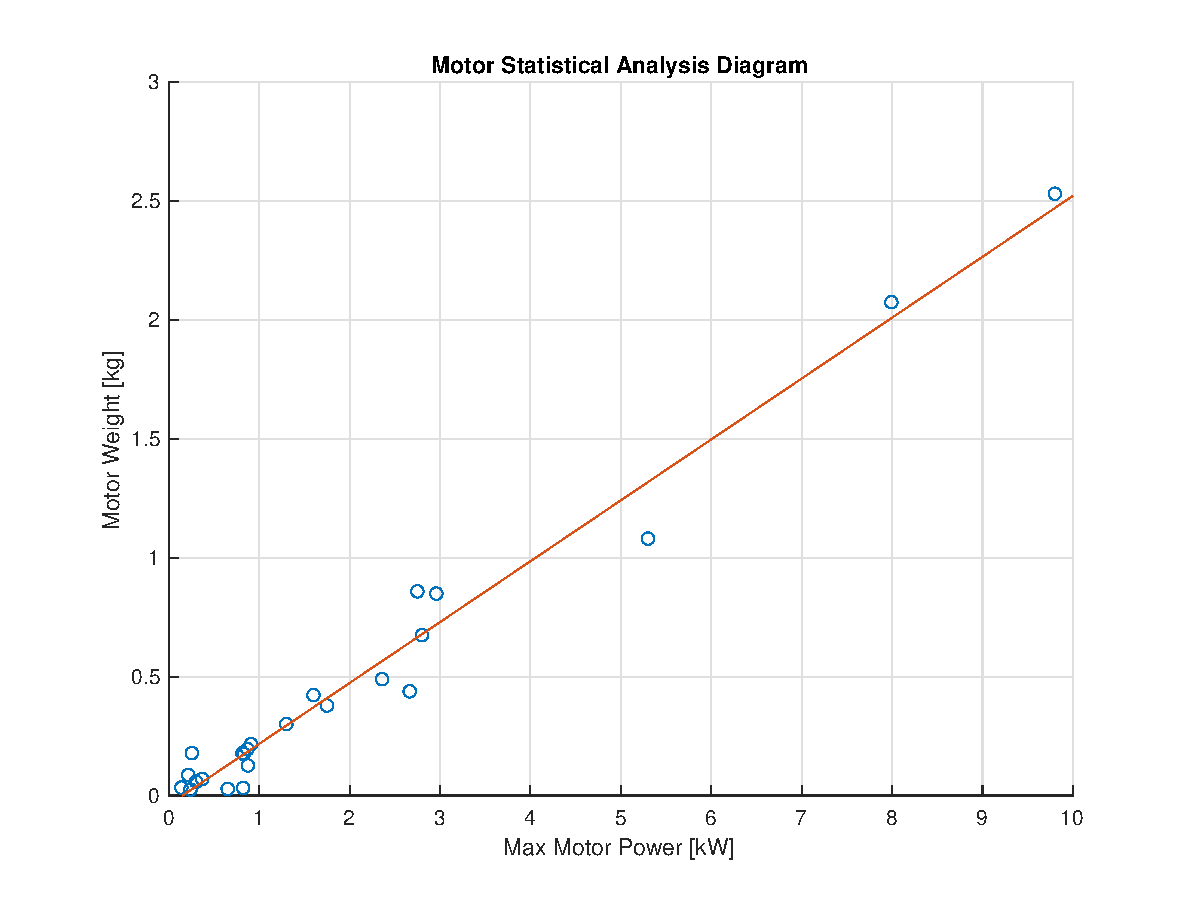
\includegraphics[width = 0.8\textwidth]{PrelimSizing/motors.eps}
    \caption{Brushless DC motor Max Power vs. Motor Weight}
    \label{fig:statmot}
\end{figure}

These values have a high degree of correlation allowing for a rough trend-line to be established, this along with the frame work detailed previously allows for an estimate of motor weight to be calculated via Equation \ref{eq:1}. 

\begin{equation}
    W_{motor} = 0.256\cdot P_{max} - 0.039
    \label{eq:1}
\end{equation}


For battery analysis, specific energy $e_{batt}$ forms the largest constraint to aircraft design. For the aircraft to complete a given mission, a fixed energy value is expended. Therefore, a battery with a greater specific energy will reduce overall weight of the drone, which in turn will reduce energy expended, increasing overall system efficiency. Another limitation of the battery is the tendency for loss of capacity over the intended life cycle. A method for prolonging battery life is to decrease the depth of discharge, however this effectively reduces the overall specific energy of the battery, therefore a battery with high specific energy and low capacity loss is preferred. For the initial sizing of this aircraft conventional lithium-ion polymer batteries (Li-po) will be selected. These have a modest specific energy of 100–265 W$\cdot$h/kg \note{CITE}{}. While this does provide some limitations, higher specific energy batteries developed in the future can be easily integrated into the existing design boosting both application and payload capabilities.  

\vspace{1cm}

Figure \ref{fig:statbatt} depicts a comparison of various COTS Li-Po batteries comparing total stored energy and battery weight. This produces a trend-line which is not linear, this can be attributed to COTS batteries including cables and a protective housing. This is more noticeable in batteries of lower weight as these auxiliary components make up less of the overall weight as total weight increases.
\begin{figure}[H]
    \centering
    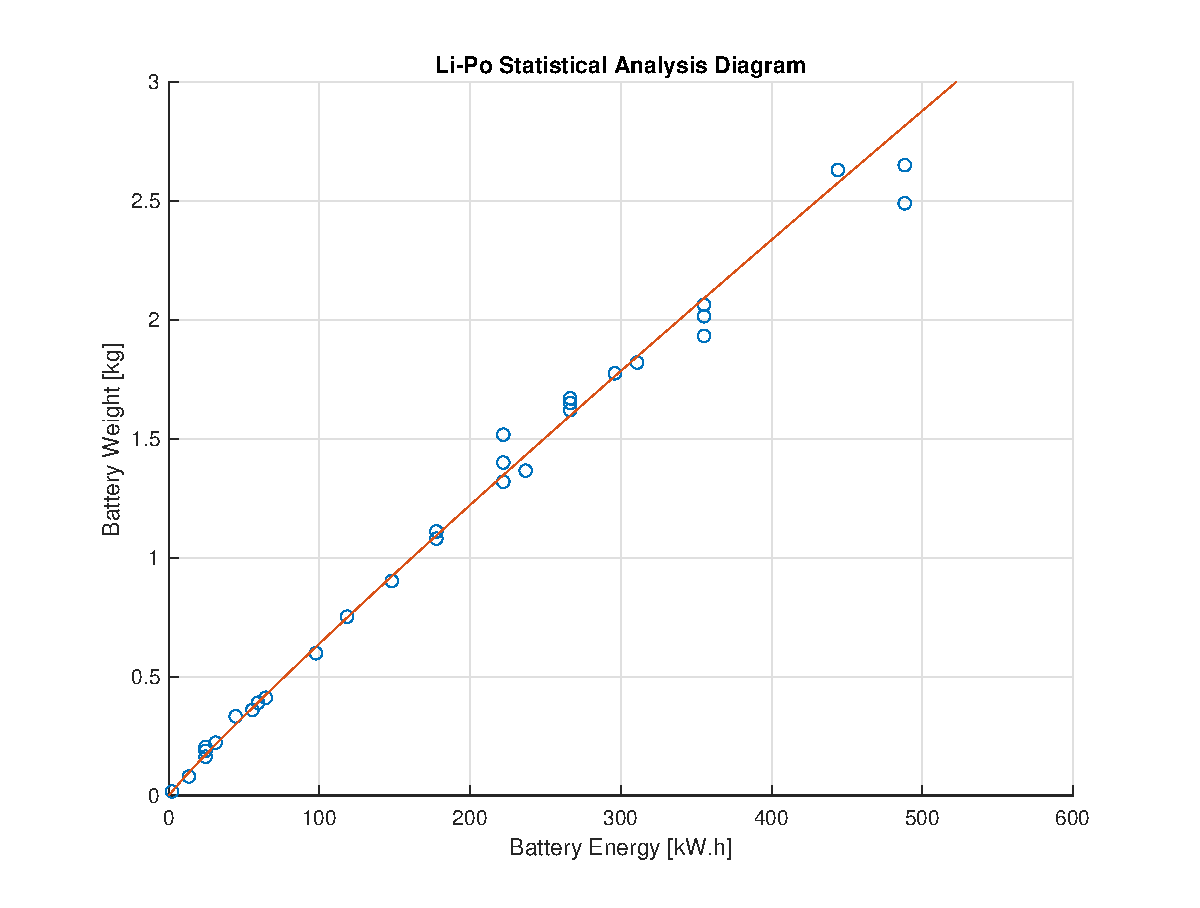
\includegraphics[width = 0.8\textwidth]{PrelimSizing/lipo.eps}
    \caption{Li-po Battery Weight vs. Total Energy}
    \label{fig:statbatt}
\end{figure}

The slope of the trend-line is equal to $1/e_{batt}$, at the higher battery weights this gives an $e_{batt}$ value of 184.45 W$\cdot$h/kg, which is comparable to literature. This analysis gives Equation \ref{eq:2}.

\begin{equation}
    W_{batt} = 0.0086\cdot E_{batt}^{0.9354}
    \label{eq:2}
\end{equation}



\paragraph{Battery Weight Analysis}

For battery weight calculations, it is defined by Equation \ref{eq:batt}. This provides a battery weight for any given specific energy and required energy. The propulsive efficiency of the system is denoted by $\eta_p$. The fraction of the battery used is represented by $F_{use}$, and determines the effective life span of the battery. More specifically, $\eta_p$ should account for efficiency losses or gains within the propulsor, motor, ESC, and current loss in connecting cables. The safety factor $SF$ considers the desired lifespan of the battery, accounting for loss of capacity. 


\begin{equation}
    W_{batt} = \dfrac{SF}{\eta_p*F_{use}} \cdot \left[ \dfrac{E_{Req}}{e_{batt}} \right]
    \label{eq:batt}
\end{equation}

If hover flight is considered, hover propulsive efficiency may be significantly different to conventional flight therefore Equation \ref{eq:batt2} is obtained.

\begin{equation}
    W_{batt} = \dfrac{SF}{F_{use}} \cdot \left[ \dfrac{\dfrac{E_{Req, FW}}{\eta_{p, FW}} + \dfrac{E_{Req, hover}}{\eta_{p, hover}}}{e_{batt}} \right]
    \label{eq:batt2}
\end{equation}

To solve this equation, values for required energy are needed for both forward and hover configurations. This was done by combining Equations \ref{eq:energy} and \ref{eq:power}.
\begin{align}
    E_{Req} &= P_{Req}\cdot t \label{eq:energy}\\
    P_{Req} &= T_{Req} \cdot v_{\infty} \label{eq:power}
\end{align}

As each flight segment has differing power requirements and duration's, mission energy requirement is given by Equation \ref{eq:missionPower}. 

\begin{equation}
    E_{Req} = \sum_{n=1}^{N} E_{Req, i}
    \label{eq:missionPower}
\end{equation}

Therefore each segments energy is given by Equation \ref{eq:segment}. 

\begin{equation}
    E_{Req, i} = \left[T_{Req, i} \cdot v_{\infty, i}\right] \cdot t_i
    \label{eq:segment}
\end{equation}

During the hover configurations of flight this equation breaks down as free-stream velocity is negligible. Therefore we must account for induced velocity produced by the propulsors. Therefore, for hover components of the mission Equation \ref{eq:hovs} is used.

\begin{equation}
    E_{Req, i, hover} = \left[T_{Req, i} \cdot \sqrt{\dfrac{T_{Req, i}}{2*A*\rho}} + v_{\infty, i}*D\right] \cdot t_i
    \label{eq:hovs}
\end{equation}



Values for segment free-stream velocity and time are given by Technical Requirement in Section 3 of this report. To find segment thrust requirements, free body analysis was conducted. It was assumed that over the span of the mission, segment transitions would be negligible, aircraft is in steady state for all mission segments, motors would idle for descent stages of flight and are not considered to have additional energy requirements. Auxiliary calculations are provided within Appendix \ref{}.


\paragraph{Empty Weight Analysis}
\note{JAKE}{Peter to write, will only be a small paragraph}


\paragraph{Constraints Analysis}
To obtain weight and power requirements found in previous sections, values for aerodynamic parameters must also be obtained. These values, such as wing area, aspect ratio, Oswald efficiency as well as lift and drag coefficients. To achieve this we need to relate weight, power and these aerodynamic parameters.\\


For conventional flight these constraints can be found using a similar process to the Roskam method \cite{roskam1985airplane} by rearranging basic lift and drag equations in terms of thrust and wing loadings. The conventional flight constraints were found for cruise, climb, stall, and flight ceiling. These are listed in Equations \ref{eq:cruise} to \ref{eq:ceiling}.
\begin{align}
    \dfrac{T}{W}_{cruise} &= q \cdot Cd_o\cdot \dfrac{S}{W}+\dfrac{k}{q}\cdot \dfrac{W}{S} \label{eq:cruise}\\
    \dfrac{T}{W}_{climb} &=  \dfrac{RC}{\cdot \sqrt{\dfrac{2}{\rho}\cdot \dfrac{W}{S}\cdot \sqrt{3\cdot Cd_o/k}}} + q \cdot Cd_o\cdot \dfrac{S}{W}+\dfrac{k}{q}\cdot \dfrac{W}{S} \label{eq:climb}\\
    \dfrac{T}{W}_{stall} &= \dfrac{1}{2}\cdot \rho \cdot v_{stall}^2 \cdot Cl_{max} \label{eq:stall}\\
    \dfrac{T}{W}_{ceiling} &= \dfrac{1}{2\cdot \sqrt{\dfrac{2}{\rho}\cdot \dfrac{W}{S}\cdot \sqrt{3\cdot Cd_o/k}}} + q \cdot \dfrac{S}{W}\cdot Cd_o + \dfrac{k}{q}\cdot \dfrac{W}{S} \label{eq:ceiling}
\end{align}

For hover, only the vertical climb segment of the flight has been considered. This is due to this segment of flight having the highest thrust and power requirements for hover configuration. This constraint is shown in Equation \ref{eq:vtolclomb}.

\begin{equation}
        \dfrac{T}{W}_{vertical climb} = SF\cdot \left(
        1 + \dfrac{1}{2}\cdot \dfrac{S}{W}\cdot V_{\infty}\cdot Cd_{V}
        \right)
    \label{eq:vtolclomb}
\end{equation}

These were then transformed to relate power loading and wing loading using Equation \ref{eq:power}. 

\begin{equation}
        \dfrac{P}{W}_{i} = \dfrac{T}{W}_{i} \cdot \dfrac{v_{\infty, i}}{\eta_{p, i}}
    \label{eq:power}
\end{equation}

From this analysis, all required information has been collected such that for a given mission, and defined technical requirements, a preliminary solution can be generated. 
\subsubsection{Results}
This analysis was mainly conducted using MATLAB, with the code found in Appendix \ref{appendixcalcs}. The results presented in this report are those of the scaled test airframe. \\

A matching diagram was generated from the constrains analysis. This diagram, depicted in Figure \ref{fig:matchingdaig}, displays the power and wing loading constraints for the aircraft. For the design to be successful it must meet all power requirements of the mission profile, this leads to a narrowing down of potential design points to those with a power loading greater then the VTOL climb constraint line. High wing loading effects an aircraft's ability to respond to gusts, its stall speed, as well reducing maneuverability. To meet mission requirements we therefore must design the aircraft with a lower wing loading then the limit imposed by its stall speed. Therefore a design area is found. From this, optimising for design requirements, A design point is selected denoted by $P_1$ on the matching diagram.

\begin{figure}[H]
    \centering
    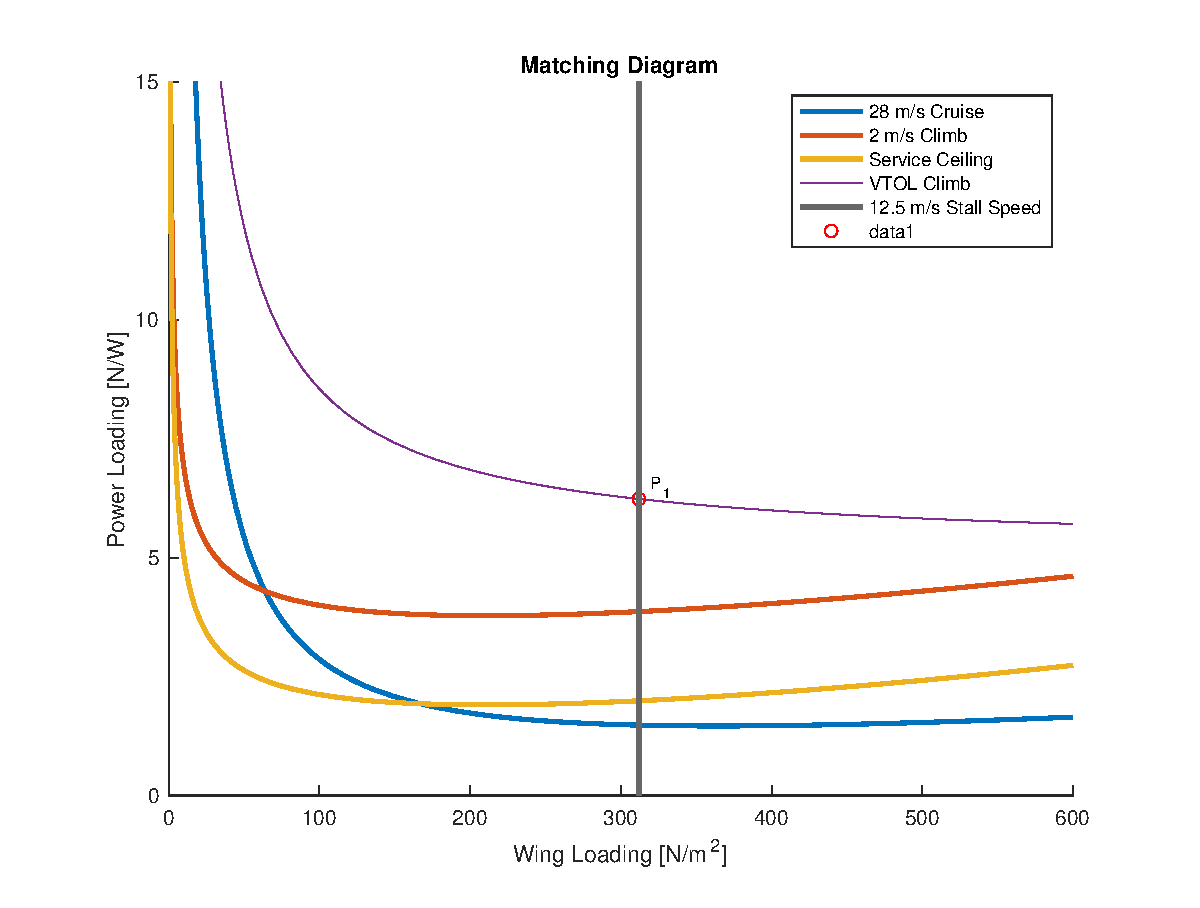
\includegraphics[width = 0.9\textwidth]{PrelimSizing/matching1.eps}
    \caption{Matching Diagram for Scaled Test Air-frame}
    \label{fig:matchingdaig}
\end{figure}

With this design point selected, analysis for the preliminary weights and aerodynamic parameters can be conducted. For convergence to occur it was found that 6 iterations were required. The preliminary values found after these 6 iterations are depicted in Table \ref{tab:preresults}.

\begin{table}[H]
\centering
\caption{Preliminary Values}
\label{tab:preresults}
\begin{tabular}{|c|c|c|}
\hline
Parameter & Value & Unit \\ \hline\hline
$M_{TOW}$ & 6.73 & $kg$ \\ \hline
$M_{Prop}$ & 0.185 & $kg$ \\ \hline
$M_{Batt}$ & 3.185 & $kg$ \\ \hline
$M_{Empty}$ & 2.36 & $kg$ \\ \hline
$M_{PL}$ & 1.00 & $kg$ \\ \hline
S & 0.6744 & $m^2$ \\ \hline
AR & 13.6 & $-$ \\ \hline
A & 0.5 & $m^2$ \\ \hline
\end{tabular}%
\end{table}

\subsubsection{Conclusion}
\note{PEter}{IDK What to put in here}



\subsubsection{Future Work}
This process is to establish preliminary values for weights and aerodynamic parameters. Moving forward with the sizing of the aircraft, it is most likely that some these values will change with detailed design. With the selection of an airframe configuration, information gained through CAD of the system such as wetted area shall be introduced into the iteration process to get more detailed estimates. From this data, aerofoils and wing geometries can be selected along with COTS batteries and motors. Stability and control considerations will also effect the final geometry of the air-frame. \\

The area of development in battery design presents great promise for the future of electric aircraft with some studies presenting novel batteries with relatively high specific energy values. A majority of these batteries are not yet commercially available, are beyond the budget of this project, or have insufficient research to justify their use. Therefore can be integrated into the design in the future as technology improves.

\clearpage
%%%%%%%%%%%%%%%%%%%%%%%%%%%%%
%\subsection{Tilt Wing}
\subsection{Tilt Wing}
%Description about it
A tilt-wing (or tilt-tail) mechanism is a common feature of numerous conceptual designs, including the two conceptual designs being pursued for prototyping.  

\subsubsection{Theory}
%What is required by the system
Tilt-wing UAVs incorporate a novel system that presents various beneficial design properties and performance merits. Research focus on developing aircraft with long-distance efficiency and VTOL capabilities has highlighted the effective use of tilt-rotors and tilt-wings by allowing motors to be used in both flight configurations, improving power efficiency and reducing unnecessary weight. Rotating the wing in parallel with the motor provides important mechanical benefits however, resulting in the tilt-wing design offering certain advantages over tilt-rotors. \\

One advantage is that the power loss due to the wings interference with propeller slipstreams is minimised. Tilt-wing design allows the slipstream from the rotor to strike the smallest possible frontal area of the wing, resulting in fewer power efficiency losses when lifting the aircraft. This is demonstrated by the V-22 Osprey tilt rotor losing about 10\% of its thrust to interference from the wings \note{(Cite)}{}. Experimental tilt-wing testing demonstrates that the total wing drag is only 4\% of the propeller thrust compared to 27\% for a tilt-rotor configuration \note{(Cite)}{}. This improved efficiency proves crucial to reducing energy consumption on small to medium scale UAVs which have inherently limited power storage. Additionally, the tilt mechanism allows control during VTOL and has the potential for control during horizontal flight. This reduces the weight and power requirements of the aircraft by eliminating the need for or reducing the size of control surfaces.\\

A tilt-wing design also has the potential to improve aerodynamics. In VTOL, the frontal area of the entire aircraft is minimised by orienting the wings such that their leading edges cut through the incoming air. Additionally, a tilt-wing mechanism can be stored within the fuselage, as opposed to common tilt motor designs which have exposed mechanisms for each rotor, adding to aerodynamic drag. \\

To ensure the advantages of a tilt-wing configuration are leveraged, a variety of VTOL and forward flight system requirements have been generated. The VTOL and forward flight configurations are illustrated in Figure \ref{fig:configs}.\\
\note{Rhys}{Does figure 16 have a box around it in the PDF?}
\begin{figure}[H]
    \centering
    \includegraphics[width = \textwidth]{Tiltwing/TiltWingConfigurations.png}
    \caption{Range of tilt-wing configurations - from left: VTOL hover, VTOL yaw, VTOL Transition, Forward Flight}
    \label{fig:configs}
\end{figure}

\paragraph{VTOL System Requirements}
In the stationary hovering state, the angle of the wings relative to the body \(\theta_w\) will be approximately \(90\degree\) (zero along the $x$-axis). For control in the VTOL configuration, the tilt mechanism must be capable of inducing a positive and negative yawing moment on the UAV. To achieve this, the wings, and therefore the thrust of the wing-mounted motors, will need to be individually actuated and have a range of rotation beyond 90\degree. The maximum achievable angle will depend on the control scheme but is unlikely to exceed 135\degree. \note{source}{} \\
\note{Rhys}{Mentions battery voltage requirement}

\paragraph{VTOL Transition System Requirements}
To achieve a controlled transition between the two flight modes, the transition phase will need to be rapid. Both wings will be required to tilt from an angle of approximately \(\theta_w=90\degree\) to approximately \(\theta_w=0\degree\) in unison and at the same rate. A separate single tilt mechanism, with rapid actuation, may be required for this.\\

\paragraph{Forward Flight System Requirements}
\note{Rhys}{Take about if the design will require 1 or 2 tilt systems and if they both have to be individually actuated}\\
To allow the tilt-wing mechanism to be utilised for control during horizontal flight, a high degree of structural integrity and rotational angle accuracy is required. A design with a reliable and stable mechanism, with minimal moving parts is therefore desired. To allow control in forward flight and to eliminate the need of additional control surfaces, both wings will be required to have a tilt angle of approximately \(\theta_w=\pm5\degree\). Furthermore, due to increased cruise velocities and generally larger forces acting on the UAV during horizontal flight to VTOL transition, the tilt mechanism must be capable of withstanding large drag induced torques. Flight forces exceeding the maximum design torque of the tilt-wing will likely result in catastrophic failure. 

\subsubsection{Methodology}
A simplified analytical approach is taken to determine the external forces and resultant moments acing on the isolated tilt-wing mechanism. Understanding the potential moments around the $y$-axis will inform the design of the mechanism by indicating the required structural integrity and informing the operational requirements of potential actuating systems such as motors or servos. Moments around the $x$-axis and the $z$-axis are not as critical to the design of the tilt mechanism as the radial and axial loads they produce can be isolated through sturdy fuselage design and effective spar support through the use of bearings.

\subsubsection{Analysis}
A reference coordinate system relative to the body of the aircraft was generated to indicate the direction of acting forces. The origin of this coordinate system is indicated as $O$, and represents the center of the main spar, not the center of mass. Additionally, it is assumed that each wing has an individual central main spar running spanwise perpendicular to the fuselage. \\

\paragraph{Forward Flight Configuration Modeling}
Figure \ref{fig:FFFBD} shows a static free body diagram of a tilt-wing during forward flight configuration. The averaged lift and drag forces of each aerofoil are functions of the linear velocities of the aircraft in the $x$ and $z$ directions, and the wing angle of attack. It is assumed that these forces act on the main spar ($y$-axis) of each wing and hence do not induce a moment around the $y$-axis at the origin. The forces produced by the port and starboard motors are assumed to act in the $x$ direction but along the $y$-axis and therefore do not produce a moment around the $y$-axis. The mass of the motors will cause a small moment around the $y$-axis, but this will likely be small compared moments cause by external disturbances such as winds and gusts.\\
\begin{figure}[H]
    \centering
    \includegraphics[width = \textwidth]{Tiltwing/FFFBD.png}
    \caption{Static Forward Flight FBD of external forces and moments acting on an isolated tilt-wing system}
    \label{fig:FFFBD}
\end{figure}

\paragraph{VTOL Configuration Modeling}
The static free body diagram of the VTOL configuration is depicted in Figure \ref{VTOLFBD}. It displays similar forces as the forward flight configuration but in different orientations with respect to the coordinate system. The averaged lift and drag forces of each aerofoil are dependent on the vertical velocity in the $z$ direction. When hovering with a constant altitude these force are zero, but will develop with increasing vertical velocity. Similarly to the forward flight configuration, these forces are assumed to act along the main spars of each wing and hence do not induce a moment around the $y$-axis.\\
\begin{figure}[H]
    \centering
    \includegraphics[width = \textwidth]{Tiltwing/VTOLFBD.png}
    \caption{Static VTOL FBD showing the external forces and moments acting on an isolated tilt-wing system}
    \label{fig:VTOLFBD}
\end{figure}

\paragraph{Worst Case Scenario Modeling}
The various forces and resultant moments of the two static configurations indicate minor torsional loads on the tilt-wing mechanism. During dynamic flight and VTOL transition the tilt mechanism will experience a larger spectrum of moments with greater amplitude. These will be created by shifting aerodynamic forces produced by the wings, external disturbances such as wind gusts and wing drag induced by VTOL transitioning. To simplify the modeling of such forces, a worst case scenario is considered. The torsional load of this scenario will occur when the aircraft suddenly transitions from forward flight to VTOL. In this scenario the two wings will quickly rotate from an angle of \(\theta_w=0\degree\) to \(\theta_w=90\degree\) relative to the body. The aerodynamic drag due to such a maneuver will induce large moments on the tilt mechanism.\\

By assuming the wings can be modeled as as a flat plate, the drag force can be calculated using Equation \ref{eqn:drag}.
\begin{equation}
    D=\frac{1}{2}C_D\rho v^2S \label{eqn:drag}
\end{equation}
% Where;
% \begin{eqnarray*}
%     C_D &=& \textnormal{coefficient of drag}\\
%     \rho &=& \textnormal{air density}\:[kg/m^3]\\
%     v &=& \textnormal{velocity of UAV}\:[m/s]\\
%     S &=& \textnormal{approximate surface area of the underside of the wing} \:[m^2]
% \end{eqnarray*}
\note{JAKE+TOM}{Rhys we need to discuss this paragraph}
The coefficient of drag is a function of several parameters including the shape of the body, Reynolds number of the flow, Froude number, Mach number and roughness of the surface. For simplification however the coefficient of drag of a flat plate perpendicular to the fluid flow was found from literature to equal 1.17. The desinsty of air is assumed to equal 1.225 \(kg/m^3\), assuming the VTOL transition occurs close to the ground. For the worse case scenario, the velocity of the UAV is found from analysis to equal 28 m/s. Lastly the approximate surface area of the underside of the wing is calculated from analysis based on the wing loading and take of weight (\ref{}). The   
\begin{gather*}
    \therefore\quad D=1.17\times \frac{1}{2}\times 1.225\times 28^2\times 0.7
\end{gather*}

\subsubsection{Results} 
\textbf{Design Requirements}\\
%talk about the torques ect determined from the modeling 
%talk about how different designs will require different servo torques
\note{Rhys}{Complete the drag calculation for the the flat plate (using aerofoil dimensions from the preliminary sizing}\\
\note{Rhys}{Calculate the moment on the tilt mechanism}\\
\\
The system requirements identified that tilt angles ranging between \(-5\degree<\theta_w<135\degree\) are required for full control in both VTOL and forward flight. Therefore the angular rotation of an actuation system must be capable of at least \(140\degree\) rotation.  \\
\\
\textbf{Actuating Motor Selection}\\
*Discuss how the tilt-wing mechanism will affect the torque required by servos etc\\
* Table of potentual servos (TS170 high torque digital RC servos with 18 kgcm torque) \\
\\
Three common motors types are considered to actuate the tilt-wing mechanism. These include; brushed and brush-less DC motors, stepper motors and positional rotation servo motors. The system requirements and design requirements are used determine which is most suitable.\\
\\
The angle of rotation required by the actuating motor must be \(140\degree\leqslant\theta_w\leqslant180\degree\). This requirement eliminates the use of brushed/brush-less DC motors which provide continuous rotation. Positional awareness with high angular accuracy is also required, supporting the use of stepper motors and DC positional rotation servo motors. Although stepper motors can accurately rotate with a high pole count ranging from 50 to 100, they too are intended for large angular rotation. Further more they have the potential to skip a pole, resulting in skewed accuracy. Their current consumption is also independent of load and hence constantly draw maximum current. DC positional rotation servos allow \(90\degree\) rotation in either direction for a total of \(180\degree\) movement, aligning well with the system requirements. A potentiometer coupled with a control circuit uses pulse width modulation (PWM) signals to control the position of the servo. This feedback system allows the servo to constantly correct any drift from the intended location. Servos are also generally able to generate higher peak torques than the holding torque of a stepper motor and are often smaller and more current efficient. In conclusion DC positional rotation servos are most applicable for the tilt-wing mechanism. \\
\\
A large range of servos with varying torque ratings, construction materials and angular speeds exist. A range of servos that meet the required torque of ??? are displayed in Table \ref{}. \\
\\
Due to the servos importance to the system, only servos with metal gears were considered as nylon gear pose the risk of stripping.\\
\\
\textbf{Preliminary Tilt Mechanism Design}\\
Based on the selection of a ??? servo, a preliminary prototype tilt-wing mechanism was designed. This prototype is a scaled version, designed to accommodate a Turnigy R5180MG analog servo. Due to the small servo size, the prototype was 3D printed for inspection and scaled operation testing. The mechanism allows for individual actuation of both wing spars, with a maximum servo rotation of \(180\degree\), easily meeting the angular rotation requirement of \(\theta_w\). Furthermore the system isolates the radial and axial loads of the wings through the use of bearings and allows for a modular wing design in which the wings can easily be detached from the system. Lastly, the mechanism can easily be modified to use one servo to actuate a single spar spanning two wings which do not require individual actuation. An isometric view of the mechanism is displayed in Figure \ref{fig:render} and additional CAD drawings can be found in Appendix \ref{}.
\begin{figure}[H]
    \centering
    \includegraphics[width = \textwidth]{Tiltwing/Tilt Assembly Render.png}
    \caption{Rendered CAD of Prototype tilt-wing Mechanism}
    \label{fig:render}
\end{figure}

\subsubsection{Conclusions}
%The moment caused by the aerodynamic drag of the vertical wings can indicate that actuating motors or servos must have a torque requirements exceeding

\subsubsection{Future Work}
Additional testing of the prototype tilt-wing mechanism is required to ensure intended functionality and full range of motion. Subject to necessary modifications, designs can then begin for a full scaled prototype. This new prototype will be scaled up to house larger ??? servos, bearings and actual wing spars. Further discussion with the workshop will also be required to discuss manufacturing difficulties and tolerances. Once the full scale prototype is complete, an iterative testing and modification stage can commence. Torque testing using a torque wrench or spring force meter will be used in this phase to test the rated holding torque of the servos and system as a whole. Once the tilt-wing mechanism is operational and near optimal, further analysis using Datcom and potentially a wind tunnel can be used to experiment with wing angles of attack to optimise the efficiency and control of the system in all flight configurations. 

%%%%%%%%%%%%%%%%%%%%%%%%%%%%
\subsection{Payload}
\label{payload}
\subsubsection{Theory} 
%SAM: It would be valuable to include a figure here to depict how these values are calculated
For a payload to fulfill its required functions there are several parameters that must be considered in its selection. For aircraft imaging payloads these are the camera pixel dimensions, field of view and aircraft altitude. To determine the spatial resolution, which is the area corresponding to one pixel, Equation \ref{eqn:Spactial} is used.\\
\begin{equation}
    \text{Spatial Resolution} = \frac{\text{Ground Area Visible}}{\text{Total Pixel Count}} \label{eqn:Spactial}
\end{equation}

\subsubsection{Method}
While the development of a payload for use by the CFS is outside the scope of this project, it is crucial that potential payloads are explored to ensure the developed system is able to incorporate the required payloads. The determining factors of payload selection are spatial resolution, weight, size and cost. 

\subsubsection{Analysis}
An analysis of 4 potential imaging systems for the payload was conducted based on the aforementioned performance criteria which is displayed in Table \ref{tab:Payloads}. 

\begin{table}[H]
\caption{Potential Payload Specification Comparisons}
\label{tab:Payloads}
\begin{tabular}{|p{3.5cm}|r|p{2.0cm}|r|r|} \hline
Imaging System  & Weight (g) & Size (mm)  & Resolution (MP) & Cost (AUD)  \\ \hline
FireFlight  & 500  & $98 \times 76 \times 68 $ & 0.3      & Unavaliable \\ \hline
GoPro (Hero 7)     & 116  & $62.3 \times 44.9 \times 33$    & 12       & 530         \\ \hline
Raspberry Pi NoIR Camera  v2 & 3.4  & \cellcolor[HTML]{FFFFFF}25 x 23 x 9   & 8     & 35   \\ \hline
Gimbal Mounted, 4k Camera    & 1000 & \cellcolor[HTML]{FFFFFF}128 x 82 x 70 & 14   & 600  \\  \hline    
\end{tabular}
\end{table}

It should be noted that the FireFlight system is a 3 camera system with two IR cameras and a single RBG camera. In addition to this, the system has integrated in flight image processing, 
Flight Path Planning and a mounting plate. Evaluating the end users needs, it was concluded that Emergency Fire Services would likely look to incorporate all 'all in one' system such as the fireflight system which has proven effectiveness on conventional fixed wing aircraft at high altitudes. Following the selection of the Fireflight system for payload integration design, the performance of the system at the maximum operating height under CASA regulations of 400ft was Investigated. Through communications with Dr Paul Dare, CEO - Fire flight, technical data for the swath width and resolution at various altitudes was acquired. The Fireflight 3000 system encompasses 3 cameras with varying focal lengths of 9mm, 13mm and 19mm. Resolutions are only provided for altitudes of 5000 ft and above and consequently the data must be extrapolated to approximate the spatial resolution at the operational altitude of 400ft\\

This was done through the determination of the Field of View (FOV) of the camera system through basic trigonometry which will allow for the calculation of the spatial resolution. The 9mm focal length case was selected as this will result in the poorest spatial resolution which if acceptable will ensure the other two camera systems are also suitable for the desired purposes.
%SAM: - An image here will be valuable in the final.
For an altitude of 5000ft, the 9mm camera system has a swath width of 1.8km. Determining the FOV angle: 
\begin{gather}
    \label{eq: FOV calculation}
    FOV = 2\times \arctan (\frac{swath\: width/2}{altitude} )\\
    FOV = 2\times \arctan ({\frac{900m}{1524m}}) = 61^o
\end{gather}
This was validated by performing the same calculations for other altitudes with a maximum calculated error of 3.5 \%. \\
Applying this FOV for an altitude of 400ft, allows the calculation of the minimum spatial resolution for the 0.3MP fireflight camera assuming a FOV of $60.0^o$.\\

\begin{gather}
    \label{eq: Swath calculation}
    Swath\: Width = altitude\times \tan(60^o)\\
    Swath\; Width = 122\times \tan(60^o) = 211m^2 \\
    Ground\: Area\: Visible = (Swath\: Width)^2 = 44521m^2 \\
    Spatial Resolution = \frac{44521m^2}{0.3\times10^6 MP} = 0.148m^2/pixel 
\end{gather}

\subsubsection{Results}
%Sam- would be good to repeat this analyse with the other 2 camera systems to determine the observable areas and resolutions for those systems
From this analysis it was observed that using the wide angle camera system a swath Width of 211m is possible, producing imagery with a spatial resolution of 0.148. This resolution should satisfy the requirements of the CFS to be able to provide valuable regarding the bushfire such as hot spots or down trees. 
\subsubsection{Discussion}
The Fireflight system was selected owing to the built in bushfire monitoring systems and proven effectiveness in this field. The system has the required resolution at the maximum operating condition. The effectiveness of the fixed wing drone due to a maximum flight altitude of 400ft may be reduced as the swath distance is insufficient to be able to accurately map vast bushfire areas. Consequently, the system may need to be paired with high altitude aircraft to further investigate identified locations of interest. Alternatively,there is the potential that drone flight restrictions may be eased as CASA continue to modify their regulations to reflect the desired uses of the aircraft which would make the aircraft far more feasible. As the Fire Flight system incorporates features which are not crucial to the drone development it will be used as a basis for the payload housing system but not practically implemented. The cost effective Pi Video camera will be used for image collection purposes.

%-What camera systems are to be Incorporated into the aircraft, Fireflight system + gopro for video recording or will this be predominantly done by the raspberry Pi cameras
\subsubsection{Conclusions}
The Fireflight Bushfire Monitoring System is a proven device that could potentially be Incorporated into the drone to achieve the needs of Emergency Fire Services. The camera achieves the required resolutions and has an acceptable size and weight. A raspberry pi camera will be integrated to the drone physically to capture appropriate video.  
-Proceeding with Fireflight camera system,
For testing purposes will use a gopro?
\subsubsection{Future Work}
Communications will continue with Fireflight to further assess the applicability of this technology to the drone. Furthermore, the payload weight will be Incorporated into the preliminary sizing calculations. The payload size specifications will be used in the development of an appropriate payload mounting system to ensure the system is able to capture the required data. 

%%%%%%%%%%%%%%%%%%%%%%%%%%%%%%%%%%%%
\clearpage

\subsection{Control - Programmable Flight Controller}

\subsubsection{Theory}
Across all prototypes, a programmable flight controller is necessary to achieve controlled VTOL and horizontal flight regimes. As supported in literature, flight controllers with PID control algorithms will be most applicable to this project. While this narrows the scope of flight controller selection, their exists numerous models which have particular advantages. Such advantages must be considered with their relevance to our performance criteria analysed.\\
\\
Among commercially available controllers, the model of processor varies depending on requirements. These models are variants of the STM32 MCU ranging from the F1 to the most recent F7 MCU which vary in processing speed and capability (REF HERE). The processor is similar to a computers CPU which evaluates computational logic and communicates with other components of the flight controller to keep the aerial system stable (REF HERE). Processing power among these different models is an imperative aspects to consider, governing the control agility and data processing capabilities of the aerial system (REF HERE).  

Through signals sent from the ground control station and those generated through the PID feedback loop on-board the flight controller, motor speed is manipulated to achieve required roll, pitch and yaw\cite{vervoorst2016modular}. Depending on the BLDC motor layout of the VTOL system, the manner in which motor speed is controlled to achieve desired motion varies \cite{vervoorst2016modular}.\\

\subsubsection{Method}

To select an optimal flight controller for this project, key aspects of programmable flight controllers will be analysed. Considerations will include price, firmware compatibility, processing power, number of UART ports and number of PWM/D-Shot input/output ports.\\
\\
A selection of popular commercially available flight controllers will be introduced and analysed against these key attributes allowing a results matrix to be formed. From this matrix, an optimal flight controller will be selected. 
\subsubsection{Analysis}
\textbf{Popular COTS Flight Controllers}\\

\textbf{Naze 32:}\\
The Naze 32 is smaller flight controller which is highly popular in the FPV multi-rotor racing society given its memory and CPU power. While this flight controller offers fast processing, support for external modules such as data collection systems and GPS modules in minimal.\\
\\
\textbf{Matek Systems F405-STD:}\\
The Matek Systems F405-STD is a highly commended flight controller given its abilities to support five UART ports and up to six PWM/Dshot outputs (REF HERE). This support makes this board ideal for GPS assisted position control while still having capabilities to support other external devices. \\

\textbf{Pixhawk Cube:}\\
The Pixhawk Cube is aimed at commercial systems where autopilot is a key requirement. This flight controller features three sets of IMU for triple redundancy, fourteen PWM outputs and five UART ports (REF HERE).\\

\textbf{Navio2:}\\
The Navio2 is vastly different from the common flight controller given its is paired with a Raspberry Pi 3 to function yielding the benefit of advanced computing power using 4 CPU cores. Furthermore, this controller promotes high end innovation such as computer vision based flight since the system is Linux based (REF HERE).\\


\subsubsection{Results}

Table \ref{tab:controller} identifies the key attributes associated with the aforementioned popular COTS flight controllers.

\begin{table}[H]
\caption{Flight Controller Selection Matrix}
\label{tab:controller}
\resizebox{\textwidth}{!}{
\begin{tabular}{|l|r|r|r|r|}
\hline
     & \textbf{Naze 32}    & \textbf{Matek F405-STD}          & \textbf{Pixhawk Cube}            & \textbf{NAVIO2}                  \\ \hline
\textbf{Price {[}AUD{]}}        & 20.12      & 47.68                   & 364.14                  & 349                     \\ \hline
\textbf{Firmware Compatability} & BaseFlight & BetaFlightArdupilotiNAV & Ardupilot               & Linux                   \\ \hline
\textbf{Processor/Clock Speed}  & F3/72MHz   & F4/168MHz               & F4/168MHz               & ARM Cortex A-53/ 1.4GHz \\ \hline
\textbf{No. UART Ports}         & 2          & 5                       & 5                       & 40                      \\ \hline
\textbf{No. PWM/Dshot Ports}    & 6 PWM      & 6 PWM/Dshot             & 14 PWM                  & 13 PWM                  \\ \hline
\textbf{Link to Objective}      & O3, O4     & O3, O4, O6, O7, O10     & O3, O4, O6, O7, O9, O10 & O3, O4, O6, O7, O9, O10 \\ \hline
\textbf{Rank}                   & 4          & 3                       & 2                       & 1                       \\ \hline
\end{tabular}}
\end{table}
\subsubsection{Discussion}
The ranking of FCs in Table~\ref{tab:controller} were determined through there suitability to the project objectives. The Naze32 FC ranked lowest given it is a heavily outdated ESC with low computational ability, thus it not suitable for high end autonomy. The Matek Systems F405-STD was more favourable given it is a later model flight controller with a higher computational speed. It was also desirable given this FCs compatibility with firmware which supports autonomous flight capabilities. Ultimately, this system provides high capabilities for a low initial costs.\\
\\
Both the Pixhawk Cube and Navio2 were closely comparable in regard to performance characteristics, however, the custom capabilities of the NAVIO32 for high end operations made this FC advantageous four this project.
\subsubsection{Summary}
As displayed in Table \ref{tab:controller}, the optimal controller for the intended prototype is the Navio2. When considering the attributes listed in Table \ref{tab:controller}, this controller is dominant and is highly applicable to this project given that the Linux environment allows for a high level of innovation in control system design and data analyses.\\

While this board is optimal, initial control system testing will use the Matek System F405-STD. This is a low-cost and effective flight control system which will allow for system integration testing of the proposed concepts before purchasing the intended flight controller. This action intends to eliminate the possibility that any control system complexities are overseen which may affect the validity of the flight controller analysis conducted above. 

\subsubsection{Future Work}
Implementation of the Matek Systems F405-STD flight controller in a simplified VTOL system will be conducted to examine whether the level of control required from the performance criteria is achievable. Any unforeseen complexities in flight control and system integration will be analysed to optimise the process of integrating the final control system into the selected prototype. 

%%%%%%%%%%%%%%%%%%%%%%%%%%%%%%%%%%%%
\subsection{Power Electronics}

\subsubsection{Theory}
%Introduce the required theory that underlines the analysis for selection of each component.
For successful flight of the proposed prototype, power electronics are required to integrate control and provide propulsion. As discussed in literature, key components include a flight controller, BLDC motors, ESCs, servo motors, a Lipo battery, data telemetry, control links and camera sensors (REF HERE). Furthermore, depending on the complexity of the mission profile, an auxiliary companion computer is required to support high level autonomy and control \cite{deci1995human}.\\
\\
Due to CASA regulations, a drone piloted under no certification can not exceed two kilograms in total flight weight \cite{CASA}. As a result, power electronics for propulsion and mechanical control will be sized to meet this regulation. Although the final manufactured prototype will exceed this weight category, a preliminary minimum complexity VTOL system will be sized and constructed allowing power electronics integration techniques to be verified.\\
\\
Of all power electronics discussed, those imperative for a minimum complexity controlled VTOL system include BLDC motors and corresponding propellers, ESCs, servo motors, a Lipo battery, control link and flight controller \cite{vervoorst2016modular}.\\
\\
When considering BLDC motor sizing, the KV rating is imperative to consider. The KV rating of a motor describes the increase in RPM per one volt increase in the supplied voltage with no load on the motor \cite{shaikh2017design}. KV rating and torque produced by the motor are inversely proportional, hence a lower KV rated motor coupled with a larger propeller will produce higher torque \cite{shaikh2017design}.\\
\\
For effective BLDC motor control, ESC selection is of high importance. The ESC module governs the voltage sent to the BLDC motor \cite{green2015modeling}. Through a PWM control signal sent from the flight controller, the ESC manipulates the duty cycle and frequency of the three phase voltage waveform, adjusting the motors speed and torque as required \cite{green2015modeling}. Commercially available ESCs come in a variety of maximum amperage sizes and corresponding switching frequencies and internal resistance \cite{green2015modeling}. Sizing of this module is performed once a BLDC motor is selected which governs the voltage required, hence maximum amperage requirement for the ESC module.\\
\\
For precise control of mechanical systems such as the tilt wing mechanism, voltage feedback servo motors provide sufficient capabilities. Through PWM signals generated from the flight controller, servo position can be precisely adjusted with a PID feedback loops. \cite{van1981motor}. When selecting servo motors for a specific application, variables such as torque to inertia ratio, speed range and peak torque are imperative to consider \cite{krishnan1987selection}. In this section, an arbitrary servo motor will be selected given the minimum complexity controlled VTOL system will not represent the forces experienced by mechanism in the final prototype.\\
\\
As discussed in previous literature, Lipo batteries provide the highest energy density, thus are most suitable for electric VTOL systems (REF HERE). After a BLDC motor is selected, with corresponding voltage requirements, a Lipo battery will be chosen. Beyond voltage requirements, Lipo batteries consist of a capacity rating and discharge rating which must be considered when sizing the power system \cite{chang2016lipo}. Battery capacity is the amount of power a battery can consistently supply given in units of Ah or mAh \cite{chuangfeng2011measurement}. Discharge rating is a relationship between battery capacity and discharge capacity denoted by C which explains the batteries maximum output current \cite{chuangfeng2011measurement}. \\
\\
The link between the operator and the VTOL system is the ground control station which is typically a combination of software and hardware to produce telemetry data \cite{haque2017drone}. Such data includes GPS location, altitude, heading, IMU data and more depending on control requirements \cite{haque2017drone}. Radio frequencies used to connect the ground control transmitter and UAV system are typically 2.4 GHZ and 5.8GHZ \cite{Radio}. These transmission frequencies are considered line-of-sight frequencies given they are not intended for long range \cite{Radio}. CASA regulations do not permit control of UAV systems beyond line of sight without certification, thus telemetry systems with higher range capability will not be considered \cite{CASALaw}. 
\subsubsection{Method}
%Follow same approach as done in the flight controller selection process: analyse COTS components against desired parameters introduced in theory.\\
In order to size an appropriate power electronics system, minimum thrust requirements will be calculated to size appropriate BLDC motors. Based on results from this analysis, corresponding components will be selected. An electrical diagram will be constructed to show the overall configuration of the power electronic components.\\
\subsubsection{Analysis}
Include calculations regarding required thrust from motors to lift a sub-2kg VTOL UAV for testing.\\
\\
Give overview of components to be considered.
\subsubsection{Results}
Provide a selection matrix for each component which reveals optimal components.
\subsubsection{Conclusions}
List the final configuration of electrical components to be further considered for testing.
\subsubsection{Future Work}
Describe methodology for testing a simplified VTOL system for analysis of component integration and theoretical analysis verification.(i.e. Is the system producing the thrust expected? Is the system actually controllable with the components selected?). 

%%%%%%%%%%%%%%%%%%%%%%%%%%%%%%%%%%%%


\subsection{Autonomous Operations}
\label{sec:autonomous}

To ensure the system is aligned with CASA regulations in accordance with Objective 2, the system will maintain constant communication with a ground based operator. The autonomous operations capability will extend to the detection of a suitable landing location and the descent of the UAV.

\subsubsection{Theory}

Based on reviewed literature, systems that use cameras to perceive the surrounding environment commonly use Python and OpenCV to perform image analysis. As described by \citeauthor{Tom5} (\citeyear{Tom5}), the three processes required for successful landing pad detection and landing are detection, tracking and displacement vector calculation. These processes will be performed by adapting existing algorithms to meet the specific needs of the application and implementing it on a micro-controller.




\subsubsection{Method}

The development of the system capable of landing site detection will be done in phases of increasing complexity.\\

An initial review of existing image segmentation algorithms will result in a system capable of simple colour and pattern detection. This can be implemented independently from the UAV and will serve as a proof of concept. Once developed, the software can be implemented using the onboard hardware.\\

Increasing the complexity of the recognition strategy will allow for more detailed perception of the environment and increase the reliability of future autonomous capabilities. As detailed in literature, it is important that the landing target can be detected and used to orient the drone when only partially visible and at varying distances. This will require the landing target detection algorithm to detect more complex shapes, and be based on more than basic colour detection.\\

% This development will verify the functionality of the 


This system will then be used as a base in which to implement and test a autonomous guidance system, ultimately capable of providing input commands to the onboard flight controller. The testing for this will be conducted by first outputting the commands to the human pilot to verify the intention of the autonomous system. After sufficient testing, the system will be set to communicate directly with the flight controller, however a human override option will always remain available.\\

The system will be required to run on a Raspberry Pi V4, using the Raspberry Pi Camera Module V2. These systems were selected as they are regularly referenced in literature as reliable components that are compatible with OpenCV.

% \subsubsection{Analysis}

% To do: Explore different algorithms for the systems

\subsubsection{Results}

An initial exploration into colour and contour detection was conducted. Using built-in functions from the OpenCV Python library, an example landing pad ($1200\times800\times3$ mm sheet of medium-density fibreboard) was detected when placed arbitrarily in a room. The raw and processed images for two angles can be seen in Figure \ref{fig:landing_detection}. 

\begin{figure}[H]
\centering
\begin{subfigure}[t]{.5\textwidth}
  \centering
  \fbox{\includegraphics[width=0.95\linewidth]{AutonomousSystems/AIML_edit.jpg}}
  \caption{Raw image 1}
%   \label{fig:cad1}
\end{subfigure}%
\begin{subfigure}[t]{.5\textwidth}
  \centering
  \fbox{\includegraphics[width=0.95\linewidth]{AutonomousSystems/AIML_edit_ctr.jpg}}
  \caption{Raw image 1 after processing}
%   \label{fig:radar1}
\end{subfigure}
\vskip\baselineskip
\begin{subfigure}[t]{.5\textwidth}
  \centering
  \fbox{\includegraphics[width=0.95\linewidth]{AutonomousSystems/AIML_edit2.jpg}}
  \caption{Raw image 2}
%   \label{fig:cad1}
\end{subfigure}%
\begin{subfigure}[t]{.5\textwidth}
  \centering
  \fbox{\includegraphics[width=0.95\linewidth]{AutonomousSystems/AIML_edit2_ctr.jpg}}
  \caption{Raw image 2 after processing}
%   \label{fig:radar1}
\end{subfigure}
\caption{Pre- and post-processing images showing landing pad detection.}
\label{fig:landing_detection}
\end{figure}

This was achieved by specifying a colour range that the landing pad fell between, and given the colour was sufficiently distinct from the rest of the space, the system was able to differentiate it from its surroundings. From the mask created by this colour filter, a contour outlining the landing pad was drawn using the \texttt{cv2.findContours()} function. This returned the coordinates of the boundary, which was then coloured green. The code used to implement this is shown in Listing \ref{code}.

\subsubsection{Discussion}
This system worked well in the controlled environment of the laboratory, where it was possible to assume constant lighting and colour palette. However, in scenarios more realistic to the application, this method alone is unlikely to be suitable due to variable environmental conditions.\\

To combat this, the landing pad should be more sophisticated. This allows it to be detected by more than its colour, which is important as it is unlikely that a single colour will be reliably distinct from its surroundings in all settings.


% \subsubsection{Conclusions}
\subsubsection{Future Work}

Further literature will be reviewed to assess which algorithms are most appropriate for the application, and after testing, the processes will be integrated to form a complete subsystem enabling autonomous landing site detection and descending onboard the UAV. This will be complete and ready to test on the manufactured prototype.\\

To extend the functionality of the system, it may be possible to look at applications of machine learning to more than landing site detection. With further information on the application desired by the CFS, the team could look at how onboard camera and computing systems could be used streamline other aspects of their operations.

%%%%%%%%%%%%%%%%%%%%%%%%%%%%%


% \section{Future Work}

\clearpage
%%%%%%%%%%%%%%%%%%%%%%%%%%%%%
\section{Summary}
This report presents the preliminary research and analysis performed on the Long Range VTOL UAV project. Motivated by the desire to develop a system capable of assisting emergency fire service endeavors, the aims and scope of the project were established. Principally the system aims to innovate in the design of a VTOL air frame and corresponding VTOL transition sequence. A minimal Viable product shall be manufactured for testing and validation purposes while further theoretical analysis will progress in parallel to allow the group to fulfill both academic and industry requirements from relevant stakeholder groups. Primary and objectives were also detailed including designing an air frame capable of operating in forward flight and hover configurations in addition to the VTOL transition and capability to perform autonomous operations.An extensive literature review provided the basis for identification of opportunities for improvements within the VTOL sector. Additionally, current marketplace solutions were assessed for each subsystem to determine the degree of integration with existing COTS systems possible.  \\

Three stages of conceptual designs were undertaken with rankings based upon qualitative analysis. Analysis the average scores of each round, improvements in meeting the specified system objectives were clearly made. Of key distinction was the propulsion system to be incorporated. Theoretical analysis was performed which displayed that the two propulsion systems were both presenting similar results meant that to distinguish between the two systems, an experimental evaluation method was desirable. Consequently, the tilt-wing mechanism was designed to be modular in the sets of wings may be attached to assess the benefits from the two proposed propulsion systems. This approach was approved by relevant stakeholders and the project scope adjusted accordingly. 
%need to speak more on prelim sizing, and individual sub system analysis, also perhaps on project managerment, safety and risk. 

\clearpage
%%%%%%%%%%%%%%%%%%%%%%%%%%%%%
\addcontentsline{toc}{section}{\protect\hphantom{\numberline{\thesection}}References}
\begin{flushleft}
\bibliographystyle{agsm}
\setcitestyle{notesep={; },round,aysep={},yysep={;}}
\bibliography{refs} % Entries are in the "refs.bib" file
\end{flushleft}

\newpage

\begin{appendices}

\section{Objective Based Performance Criteria}
\label{app_performance_criteria}

Tables \ref{tab:obj_1_criteria} to \ref{tab:obj_6_criteria} detail the performance criteria used to compare the airframe concepts generated during the ideation stage of the project. These criteria were developed using the Specific, Relevant, Measurable and Scalable framework.

% \begin{table}[ht]
% \vspace{-1.25cm}
% \caption{Performance Criteria for Objectives}
% \vspace{-0.25cm}
% \label{performance-criteria}
% \centering
% \resizebox{1.4\textwidth}{!}{
% \begin{tabular}{|p{3cm}|p{8cm}|p{10cm}|p{10cm}|p{10cm}|p{12cm}|p{2cm}|}
% \hline
%     \textbf{Objectives} & \textbf{Criteria} & \textbf{Description} & \textbf{Measurable} & \textbf{Bad = 1} & \textbf{Good = 10} & \textbf{Weighting} \\ \hline \hline
%     \#1 & Ease of manufacturing & How difficult it is to manufacturer the design. & Predicted manufacturing time, requires external sourcing, tool types required & unable to be manufactured by group/external manufacturer & Easily manufactured without external sourcing and within time frame & 0.25 \\ \hline
% 	 & Durability & The ability of the airframe to withstand a failure and crash. Level of maintenance. & Delicate parts, external components, materials, & Delicate external parts & Exterior offers crash protection to important subsystems & 0.1 \\ \hline
% 	 & Reliability & How reliable the airframe design in regards to comparing to standard airframe design. & Basis of design, No. of actuators, No. of Control Surfaces, Effectiveness of Control Surfaces  & no past designs to base off & Minimal complex parts, with large control surfaces & 0.2 \\ \hline
% 	 & Availability of materials & How accessible the airframe's designed materials are. & Delivery time/access time & Materials/parts are readily available in workshops & Materials/parts are sourced from overseas with delivery times exceeding a month & 0.1 \\ \hline
% 	 & Ease of assembly / design complexity & The difficulty of manufacturing and assembling the airframe's design. & number of parts, Modularity, Fastener Type & Excessive number of parts with complicated connections & Mimimal number of parts with simple connection interfaces & 0.05 \\ \hline
% 	 & Ease of transport & The difficulty assoicated with transporting the airframe's design once manfactured. & Modulal design & Requires & Simply Transportable in Common Car & 0.05 \\ \hline
% 	 & Weight & The airframe design's expected weight. & assembled weight (including batteries without payload) & Heavy Airframe, outside of allocated weight allowance & Falls within Allocated Weight Range, Reasonably Light & 0.15 \\ \hline
% 	 & Cost & The total cost to manufacture the airframe's design. & Procurement cost, manufacturing cost & Exceeds Allocated Budget & New Project Costs under budget & 0.1 \\ \hline
% 	\#3 & Forward Aerodynmaic efficiency (forward flight L/D) & How amount of lift versus drag produced during forward flight. & The total lift of the aircraft compaired to the total drag & Low lift to drag ratio & High lift to drag ratio & 0.22 \\ \hline
% 	 & Propulsive Efficency (Eta\_p\_f) & Propulsive efficiency achieved during level flight. & The efficency of thrust power out compaired to power input &  &  & 0.16 \\ \hline
% 	 & Max Forward Flight Endurance & The maximum endurance range the aicraft can achieve purely in forward flight. & Distance acheiveable by the device & Can't operate & Can operate indefinetly in a forward flight confiuration & 0.15 \\ \hline
% 	 & Operational altitude & The altitude range which the aircraft can operate when in forward flight. & Per Description & Requires Operational Flight at an altitude above CASA regulations & Can operate at all altitudes up to 400ft AGL & 0.05 \\ \hline
% 	 & Controlability & The amount of control the pilot has over the aircraft's yaw, pitch and roll when in forward flight. & Number of control surfaces required, effectiveness of control surfaces & The pilot has zero control & device was low response time to pilot commands, low overshoot, high precision & 0.05 \\ \hline
% 	 & power usage & Required power consumption for forward flight. & Power to weight ratio & Low power to weight ratio (1:1) & High power to weight power (4:1) & 0.12 \\ \hline
% 	 & Speed controlability/range & The operational speed range and ability to control speed output. & Forward flight operational range & Zero speed controlability. & Low speed range during horizontal flight without stall. Large speed range for both vertical and horizontal flight. & 0.1 \\ \hline
% 	 & Stability (abilty to handle gusts ect) & The aircraft's stability when in forward flight, and how easy it is to maintain and return to. & Is the aircraft statically stable, stability in other directional planes, ability to handle gusts. & Device can only operate in still wind conditions & Device can operate during wind conditions typical for a catastropic fire danger day & 0.1 \\ \hline
% 	 & Redundancy & The aircrafts failsafe ability & Devices ability to sustain flight during/after a failure. Number of backup or fail-safe systems. & Zero redundancy. Small failures cause a critical device failure & Multiple reduncancy with back-up components and fail-safe measures for both horizonatal and verical flight & 0.05 \\ \hline
% 	\#4 & Vertical Aerodynmaic efficiency ((T+L)/W) & The aerodynamic efficiency of the aircraft in the vertical configuration & The total lift + thurst of the aircraft compaired to the total drag in vertical configuration & low ratio & high ratio & 0.1 \\ \hline
% 	 & Propulsive Efficency (Eta\_p\_v) & The propulsive efficiency achieved during vertical flight. & The efficency of thrust power out compaired to power input & Low efficency (<40\%) & High effciency (>80\%) & 0.2 \\ \hline
% 	 & Max Hover Endurance & The maximum time that a device can operate in the hovor configuration & The time the in minuites that the device can hovor for & Hovor endurance not sufficient to reach operational height & Hovor efficiency can completely satisfy mission profile & 0.09 \\ \hline
% 	 & Operational altitude & The altitude range which the aircraft can operate at when in hover. & The altitude range in meters where the device can operate at & Requires Operational Flight at an altitude above CASA regulations & Can operate at all altitudes up to 400ft AGL & 0.02 \\ \hline
% 	 & Controlability & The amount of control the aircraft has in yaw, pitch and roll when in vertical flight. & Number of control surfaces required, effectiveness of control surfaces & Device cannot be controlled in hovor configuration & The device can remain stationary in all axis, and ascend and descend in 1 axis & 0.16 \\ \hline
% 	 & Power useage & The power required to operate in a hovour configuration & The battery capacity dissipated in hover 
% configuration for expected time in loitering
% phase of mission profile & >20\% & Capable of sustainig 10 hovor configurations as per mission profile & 0.05 \\ \hline
% 	 & Speed controlability/range & Range of speed that the drone can be controlled at & How slow / fast can the system move vertically. Control at low and high speed is important. & Controlable only for one speed & Controlable for +/- 50\% of average speed & 0.1 \\ \hline
% 	 & Hover stability (abilty to handle gusts ect) & The aircraft's stability when in hover or vertical flight, and how easy it is to maintain and return to. & Is the aircraft statically stable, stability in other planes. & Device can only operate in still wind conditions & Device can operate during wind conditions typical for a catastropic fire danger day & 0.18 \\ \hline
% 	 & Landing gear & A component which protects the airframe in takeoff and landing & The force the landing gear can support before fail & Landing gear cannot sustain forces in standard takeoff and landing & Landing gear that can handle variable landing conditions and ground terrain. Is multipurpose and does not increase drag & 0.05 \\ \hline
% 	 & Redundancy & The aircrafts failsafe ability & Devices ability to sustain flight during/after a failure. Number of backup or fail-safe systems. & Zero redundancy. Small failures cause a critical device failure & Multiple reduncancy with back-up components and fail-safe measures for both horizonatal and verical flight & 0.05 \\ \hline
% 	\#5 & Ease of payload insertion, & The simplicity and ease to insert payload into the system & Does it require tools, tool complexity, time required to insert the payload, how obvious is it that its inserted & Requires complicated tools, and has a loose fit & Requires no tools and clicks in obviously & 0.15 \\ \hline
% 	 & size and size range of potential payload, & The volume of the payload, as well as how that volume is distributed & Cubic centemetres & It doesnt accept a payload & Payload can by up to 50\% of weight & 0.1 \\ \hline
% 	 & weight and weight range of payload, & The mass in Kg of the paylaod that the vehicle can safely carry, This shouldnt effect the stability or controllibility of the aircraft in any meaningful way & Kilograms & Too heavy for 
% airframe to support & Little infrastructure 
% required to support
% payload & 0.18 \\ \hline
% 	 & Payload impact on flight & The impacts created by the payload when installed, such as increased drag or is the payload integrated to minimise flight impacts. & Flight time. Drag Force [N] & Payload greatly influences size of frontal area & Payload has minimal effect on frontal area of aiframe adding little drag & 0.3 \\ \hline
% 	 & damage mitigration (vuntrability), & The payloads resistance to damage if failure of the system occurs & How far does payload protrude from body & Payload is external to airframe & Payload is within the main profile & 0.04 \\ \hline
% 	 & payload orientation (operation affected by hover/horizontal flight) & The effect different orientations has on the payload to complete objectives & How many different types of data can be collected from each orientation - how many orietations are their? & The payload is unable to collect meaningfull data & The payload is able to collect all nessesary data, regardless of orientation & 0.23 \\ \hline
% 	\#6 & Transition time & The time it takes to transition to other flight mode & Seconds & Takes longer than 10 seconds & Takes no time to transition & 0.08 \\ \hline
% 	 & Transition Efficiency & The ammount of battery capacity dissipated 
% in transition phase & Battery Capacity Dissipated \% & >10\% & <5\% & 0.16 \\ \hline
% 	 & Transition Complexity & The complexity of control systems required to transitions & Requirement for custom flight control dynamics & Requires custom flight control dynamics & Standard in cheap COTS systems & 0.13 \\ \hline
% 	 & Transition Unique Components & Components that are only used in one configuration, and therefore are deadweight in the auxilery configuration & Weight spent on transition unique components, number of actuators required & 10\% of aircraft weight is on transition unique components & No specific systems for transition & 0.12 \\ \hline
% 	 & Spatial requirments for tranisiton (altitude, area etc) & The altitude, airspace, and other limiations that effect when trasition can occur & Altitude required [m] & System requires =>30 metres for transition & System looses zero altitude during transistion & 0.11 \\ \hline
% 	 & Reliability of Transition & The ability for the aircraft to have a high success of transition. & Percentage of successful transitions based on physical testing & <90 & >95 & 0.15 \\ \hline
% 	 & Trasition Robustness & The ability for the aircarft to transition in various weather conditions including but not limited to, gusts, crosswinds, density, etc & Maximum cross-wind speed that system can performVTOL transition [kts] & The system can only transition with cross-winds less then 10 kts & The system can transistion with 40 kts cross-winds & 0.15 \\ \hline
% 	 & Redundancy (what if something goes wrong during transition) & If there is a motor of actuator failure, can the system land or continue flying & Number of actuators or motors that can fail before the system is uncontrollerable & No redundancy systems & Can land in a controlled manner or continue in former flight mode in the event of motor or actuator failure & 0.1 \\ \hline
% \end{tabular}}
% \end{table}


%%%%%%%%%%%%%%%%%%%%%%%%%%%%%%%%%%%%%%%%%%%%%%%%%%%%%%%%
% Objective 1
%%%%%%%%%%%%%%%%%%%%%%%%%%%%%%%%%%%%%%%%%%%%%%%%%%%%%%%%


\begin{table}[H]
\centering
\caption{Performance Criteria for Objective 1: Design and Manufacture an Airframe}
\label{tab:obj_1_criteria}
\resizebox{\textwidth}{!}{%
\begin{tabular}{|p{2cm}|p{4cm}|p{4cm}|p{4cm}|p{4cm}|r|}
\hline
\textbf{Criteria}                             & \textbf{Description}                                                                           & \textbf{Measurable}                                                                                            & \textbf{Bad = 1}                                                  & \textbf{Good = 10  }                                                                     & \textbf{Weighting} \\ \hline
Ease of manufacturing                & How difficult it is to manufacturer the design.                                       & Predicted manufacturing time, requires external sourcing, tool types required                         & Unable to be manufactured by group/external manufacturer & Easily manufactured without external sourcing and within time frame             & 0.25      \\ \hline
Durability                           & The ability of the airframe to withstand a failure and crash. Level of maintenance.   & Delicate parts, external components, materials,                                                       & Delicate external parts                                  & Exterior offers crash protection to important subsystems                        & 0.1       \\ \hline
Reliability                          & How reliable the airframe design in regards to comparing to standard airframe design. & Basis of design, number. of actuators, number. of Control Surfaces, Effectiveness of Control Surfaces & Number past designs to base off                          & Minimal complex parts, with large control surfaces                              & 0.2       \\ \hline
Availability of materials            & How accessible the airframe's designed materials are.                                 & Delivery time/access time                                                                             & Materials/parts are readily available in workshops       & Materials/parts are sourced from overseas with delivery times exceeding a month & 0.1       \\ \hline
Ease of assembly / design complexity & The difficulty of manufacturing and assembling the airframe's design.                 & number of parts, Modularity, Fastener Type                                                            & Excessive number of parts with complicated connections   & Minimal number of parts with simple connection interfaces                       & 0.05      \\ \hline
Ease of transport                    & The difficulty associated with transporting the airframe's design once manufactured.  & Assembled weight (including batteries without payload)                                                & Cannot be transported                                                 & Simply Transportable in Common Car                                              & 0.05      \\ \hline
Weight                               & The airframe design's expected weight.                                                & Assembled weight (including batteries without payload)                                                & Heavy Airframe, outside of allocated weight allowance    & Falls within Allocated Weight Range, Reasonably Light                           & 0.15      \\ \hline
Cost                                 & The total cost to manufacture the airframe's design.                                  & Procurement cost, manufacturing cost                                                                  & Exceeds Allocated Budget                                 & New Project Costs under budget                                                  & 0.1       \\ \hline
\end{tabular}%
}
\end{table}



%%%%%%%%%%%%%%%%%%%%%%%%%%%%%%%%%%%%%%%%%%%%%%%%%%%%%%%%
% Objective 2
%%%%%%%%%%%%%%%%%%%%%%%%%%%%%%%%%%%%%%%%%%%%%%%%%%%%%%%%

% Please add the following required packages to your document preamble:
% \usepackage{graphicx}
\begin{table}[H]
\centering
\caption{Performance Criteria for Objective 2: Design Complies with Standards and Regulations}
\label{tab:obj_2_criteria}
\resizebox{\textwidth}{!}{%
\begin{tabular}{|p{2cm}|p{4cm}|p{4cm}|p{4cm}|p{4cm}|r|}
\hline
\textbf{Criteria}      & \textbf{Description}                                                                                         & \textbf{Measurable}                                                 & \textbf{Bad = 1}                                                                  & \textbf{Good = 10}                                                       & \textbf{Weighting} \\ \hline
Flight zone            & CASA approved flight grounds                                                                                 & Seeking approval to test on flight grounds                          & Cannot meet approval requirements                                                 & Design meets required criteria                                           & -                  \\ \hline
Weight category        & CASA regulated weight category                                                                               & 2- 25kg (to checked)                                                & Device exceeds 25kg, not adhering to regulation and cannot be flown               & Design meets required criteria                                           & -                  \\ \hline
Autonomy requirement   & Does it require autonomy to fly. dependence on autonomy is a bad thing in terms of getting permission to fly & Number of autonomous systems, dependence on these systems           & Is completely autonomous with no human fail-safe                                  & Design does not impose additional requirements due to autonomous feature & -                  \\ \hline
Altitude requirement   & The maximum operational altitude of the aircraft to comply with CASA.                                        & 400 ft altitude limit (to be confirmed)                             & Device cannot operate under 400ft, not adhering to regulation and cannot be flown & Can operate at all altitudes below 400ft                                 & -                  \\ \hline
Flight Pilot Available & How difficult it is to locate a pilot with the required approval to fly the UAV.                             & Ease of finding Individual with appropriate operational certificate & Device cannot be flown by any accredited UAV pilots                               & Persons with no qualifications can fly the UAV                           & -                  \\ \hline
\end{tabular}%
}
\end{table}





%%%%%%%%%%%%%%%%%%%%%%%%%%%%%%%%%%%%%%%%%%%%%%%%%%%%%%%%
% Objective 3
%%%%%%%%%%%%%%%%%%%%%%%%%%%%%%%%%%%%%%%%%%%%%%%%%%%%%%%%



% Please add the following required packages to your document preamble:
% \usepackage{graphicx}
\begin{table}[H]
\centering
\caption{Performance Criteria for Objective 3: Design System Capable of Forward Flight}
\label{tab:obj_3_criteria}
\resizebox{\textwidth}{!}{%
\begin{tabular}{|p{2cm}|p{4cm}|p{4cm}|p{4cm}|p{4cm}|r|}
\hline
\textbf{Criteria}                                            & \textbf{Description}                                                                                         & \textbf{Measurable}                                                                                         & \textbf{Bad = 1}                                                           & \textbf{Good = 10}                                                                                                        & \textbf{Weighting} \\ \hline
Forward Aerodynamic efficiency (forward flight L/D) & How amount of lift versus drag produced during forward flight.                                      & The total lift of the aircraft compared to the total drag                                          & Low lift to drag ratio                                            & High lift to drag ratio                                                                                            & 0.22      \\ \hline
Propulsive Efficiency (Eta\_p\_f)                   & Propulsive efficiency achieved during level flight.                                                 & The efficiency of thrust power out compared to power input                                         &                                                                   &                                                                                                                    & 0.16      \\ \hline
Max Forward Flight Endurance                        & The maximum endurance range the aircraft can achieve purely in forward flight.                      & Distance achievable by the device                                                                  & Can't operate                                                     & Can operate indefinitely in a forward flight configuration                                                         & 0.15      \\ \hline
Operational altitude                                & The altitude range which the aircraft can operate when in forward flight.                           & Per Description                                                                                    & Requires Operational Flight at an altitude above CASA regulations & Can operate at all altitudes up to 400ft AGL                                                                       & 0.05      \\ \hline
Flight Controllability                                     & The amount of control the pilot has over the aircraft's yaw, pitch and roll when in forward flight. & Number of control surfaces required, effectiveness of control surfaces                             & The pilot has zero control                                        & device was low response time to pilot commands, low overshoot, high precision                                      & 0.05      \\ \hline
Power usage                                         & Required power consumption for forward flight.                                                      & Power to weight ratio                                                                              & Low power to weight ratio (1:1)                                   & High power to weight power (4:1)                                                                                   & 0.1       \\ \hline
Speed controllability/range                         & The operational speed range and ability to control speed output.                                    & Forward flight operational range                                                                   & Zero speed controllability.                                       & Low speed range during horizontal flight without stall. Large speed range for both vertical and horizontal flight. & 0.1       \\ \hline
Stability (ability to handle gusts etc)             & The aircraft's stability when in forward flight, and how easy it is to maintain and return to.      & Is the aircraft statically stable, stability in other directional planes, ability to handle gusts. & Device can only operate in still wind conditions                  & Device can operate during wind conditions typical for a catastrophic fire danger day                               & 0.1       \\ \hline
Redundancy                                          & The aircraft's fail-safe ability                                                                      & Devices ability to sustain flight during/after a failure. Number of backup or fail-safe systems.   & Zero redundancy. Small failures cause a critical device failure   & Multiple redundancy with back-up components and fail-safe measures for both horizontal and vertical flight         & 0.05      \\ \hline
\end{tabular}%
}
\end{table}



%%%%%%%%%%%%%%%%%%%%%%%%%%%%%%%%%%%%%%%%%%%%%%%%%%%%%%%%
% Objective 4
%%%%%%%%%%%%%%%%%%%%%%%%%%%%%%%%%%%%%%%%%%%%%%%%%%%%%%%%



% Please add the following required packages to your document preamble:
% \usepackage{graphicx}
\begin{table}[H]
\centering
\caption{Performance Criteria for Objective 4: Design System Capable of Hovering}
\label{tab:obj_4_criteria}
\resizebox{\textwidth}{!}{%
\begin{tabular}{|p{2cm}|p{4cm}|p{4cm}|p{4cm}|p{4cm}|r|}
\hline
\textbf{Criteria}                                      & \textbf{Description}                                                                                              & \textbf{Measurable}                                                                                                                                                  & \textbf{Bad = 1}                                                             & \textbf{Good = 10}                                                                                                               & \textbf{Weighting} \\ \hline
Vertical Aerodynamic efficiency ((T+L)/W)     & The aerodynamic efficiency of the aircraft in the vertical configuration                                 & The total lift and thrust of the aircraft compared to the total drag in vertical configuration                                                                & low ratio                                                           & high ratio                                                                                                              & 0.1       \\ \hline
Propulsive Efficiency (Eta\_p\_v)             & The propulsive efficiency achieved during vertical flight.                                               & The efficiency of thrust power out compared to power input                                                                                                  & Low efficiency (\textless{}40\%)                                    & High efficiency (\textgreater{}80\%)                                                                                    & 0.2       \\ \hline
Max Hover Endurance                           & The maximum time that a device can operate in the hover configuration                                    & The time the in minutes that the device can hover for                                                                                                       & Hover endurance not sufficient to reach operational height          & Hover efficiency can completely satisfy mission profile                                                                 & 0.09      \\ \hline
Operational altitude                          & The altitude range which the aircraft can operate at when in hover.                                      & The altitude range in meters where the device can operate at                                                                                                & Requires Operational Flight at an altitude above CASA regulations   & Can operate at all altitudes up to 400ft AGL                                                                            & 0.02      \\ \hline
Hover controllability                         & The amount of control the aircraft has in yaw, pitch and roll when in vertical flight.                   & Number of control surfaces required, effectiveness of control surfaces                                                                                      & Device cannot be controlled in hover configuration                  & The device can remain stationary in all axis, and ascend and descend in 1 axis                                          & 0.16      \\ \hline
Power usage                                   & The power required to operate in a hover configuration                                                   & The battery capacity dissipated in hover configuration for expected time in loitering phase of mission profile & \textgreater{}20\%                                                  & Capable of sustaining 10 hover configurations as per mission profile                                                    & 0.05      \\ \hline
Speed controllability/range                   & Range of speed that the drone can be controlled at                                                       & How slow / fast can the system move vertically. Control at low and high speed is important.                                                                 & Controllable only for one speed                                     & Controllable for +/- 50\% of average speed                                                                              & 0.1       \\ \hline
Hover stability (ability to handle gusts etc) & The aircraft's stability when in hover or vertical flight, and how easy it is to maintain and return to. & Is the aircraft statically stable, stability in other planes.                                                                                               & Device can only operate in still wind conditions                    & Device can operate during wind conditions typical for a catastrophic fire danger day                                    & 0.18      \\ \hline
Landing gear                                  & A component which protects the airframe in take-off and landing                                          & The force the landing gear can support before fail                                                                                                          & Landing gear cannot sustain forces in standard take-off and landing & Landing gear that can handle variable landing conditions and ground terrain. Is multipurpose and does not increase drag & 0.05      \\ \hline
Redundancy                                    & The aircraft's fail-safe ability                                                                           & Devices ability to sustain flight during/after a failure. Number of backup or fail-safe systems.                                                            & Zero redundancy. Small failures cause a critical device failure     & Multiple redundancy with back-up components and fail-safe measures for both horizontal and vertical flight              & 0.05      \\ \hline
\end{tabular}%
}
\end{table}



%%%%%%%%%%%%%%%%%%%%%%%%%%%%%%%%%%%%%%%%%%%%%%%%%%%%%%%%
% Objective 5
%%%%%%%%%%%%%%%%%%%%%%%%%%%%%%%%%%%%%%%%%%%%%%%%%%%%%%%%

% Please add the following required packages to your document preamble:
% \usepackage{graphicx}
% \usepackage[normalem]{ulem}
% \useunder{\uline}{\ul}{}
\begin{table}[H]
\centering
\caption{Performance Criteria for Objective 5: Design a System with Payload Capacity}
\label{tab:obj_5_criteria}
\resizebox{\textwidth}{!}{%
\begin{tabular}{|p{2cm}|p{4cm}|p{4cm}|p{4cm}|p{4cm}|r|}
\hline
\textbf{Criteria}                                                            & \textbf{Description}                                                                                                                                                   & \textbf{Measurable}                                                                                                       & \textbf{Bad = 1}                                                                      & \textbf{Good = 10}                                                                                      & \textbf{Weighting} \\ \hline
Ease of payload insertion,                                          & The simplicity and ease to insert payload into the system                                                                                                     & Does it require tools, tool complexity, time required to insert the payload, how obvious is it that its inserted & Requires complicated tools, and has a loose fit                              & Requires no tools and clicks in obviously                                                      & 0.15      \\ \hline
size and size range of potential payload,                           & The volume of the payload, as well as how that volume is distributed                                                                                          & Cubic centimetres                                                                                                & It doesn't accept a payload                                                  & Payload can by up to 50\% of weight                                                            & 0.1       \\ \hline
weight and weight range of payload,                                 & The mass in Kg of the payload that the vehicle can safely carry, This shouldn't effect the stability or controllability of the aircraft in any meaningful way & Kilograms                                                                                                        & Too heavy for airframe to support & Little infrastructure required to support payload & 0.18      \\ \hline
Payload impact on flight                                            & The impacts created by the payload when installed, such as increased drag or is the payload integrated to minimise flight impacts.                            & Flight time. Drag Force {[}N{]}                                                                                  & Payload greatly influences size of frontal area                              & Payload has minimal effect on frontal area of airframe adding little drag                      & 0.3       \\ \hline
damage mitigation (vulnerability),                                  & The payloads resistance to damage if failure of the system occurs                                                                                             & How far does payload protrude from body                                                                          & Payload is external to airframe                                              & Payload is within the main profile                                                             & 0.04      \\ \hline
payload orientation (operation affected by hover/horizontal flight) & The effect different orientations has on the payload to complete objectives                                                                                   & How many different types of data can be collected from each orientation - how many orientations are their?       & The payload is unable to collect meaningful data                             & The payload is able to collect all necessary data, regardless of orientation                   & 0.23      \\ \hline
\end{tabular}%
}
\end{table}



%%%%%%%%%%%%%%%%%%%%%%%%%%%%%%%%%%%%%%%%%%%%%%%%%%%%%%%%
% Objective 6
%%%%%%%%%%%%%%%%%%%%%%%%%%%%%%%%%%%%%%%%%%%%%%%%%%%%%%%%



% Please add the following required packages to your document preamble:
% \usepackage{graphicx}
% \usepackage[normalem]{ulem}
% \useunder{\uline}{\ul}{}
\begin{table}[H]
\centering
\caption{Performance Criteria for Objective 6: Design System to Perform VTOL Transitions}
\label{tab:obj_6_criteria}
\resizebox{\textwidth}{!}{%
\begin{tabular}{|p{2cm}|p{4cm}|p{4cm}|p{4cm}|p{4cm}|r|}
\hline
\textbf{Criteria}                                                    & \textbf{Description}                                                                                                                            & \textbf{Measurable}                                                                      & \textbf{Bad = 1   }                                                       &\textbf{ Good = 10 }                                                                                                  & \textbf{Weighting} \\ \hline
Transition time                                             & The time it takes to transition to other flight mode                                                                                   & Seconds                                                                         & Takes longer than 10 seconds                                     & Takes no time to transition                                                                                 & 0.08      \\ \hline
Transition Efficiency                                       & The amount of battery capacity dissipated in transition phase                           & Battery Capacity Dissipated \%                                                  & \textgreater{}10\%                                               & \textless{}5\%                                                                                              & 0.16      \\ \hline
Transition Complexity                                       & The complexity of control systems required to transitions                                                                              & Requirement for custom flight control dynamics                                  & Requires custom flight control dynamics                          & Standard in cheap COTS systems                                                                              & 0.13      \\ \hline
Transition Unique Components                                & Components that are only used in one configuration, and therefore are deadweight in the auxiliary configuration                        & Weight spent on transition unique components, number of actuators required      & 10\% of aircraft weight is on transition unique components       & No specific systems for transition                                                                          & 0.12      \\ \hline
Spatial requirements for transition (altitude, area etc)    & The altitude, airspace, and other limitations that effect when transition can occur                                                    & Altitude required {[}m{]}                                                       & System requires =\textgreater{}30 metres for transition          & System looses zero altitude during transition                                                               & 0.11      \\ \hline
Reliability of Transition                                   & The ability for the aircraft to have a high success of transition.                                                                     & Percentage of successful transitions based on physical testing                  & \textless{}90                                                    & \textgreater{}95                                                                                            & 0.15      \\ \hline
Transition Robustness                                       & The ability for the aircraft to transition in various weather conditions including but not limited to, gusts, crosswinds, density, etc & Maximum cross-wind speed that system can perform VTOL transition {[}kts{]}      & The system can only transition with cross-winds less then 10 kts & The system can transition with 40 kts cross-winds                                                           & 0.15      \\ \hline
Redundancy (what if something goes wrong during transition) & If there is a motor of actuator failure, can the system land or continue flying                                                        & Number of actuators or motors that can fail before the system is uncontrollable & No redundancy systems                                            & Can land in a controlled manner or continue in former flight mode in the event of motor or actuator failure & 0.1       \\ \hline
\end{tabular}%
}
\end{table}



%%%%%%%%%%%%%%%%%%%%%%%%%%%%%%%%%%%%%%%%%%%%%%%%%%%%%%%%
% Objective 7
%%%%%%%%%%%%%%%%%%%%%%%%%%%%%%%%%%%%%%%%%%%%%%%%%%%%%%%%


% Please add the following required packages to your document preamble:
% \usepackage{graphicx}
% \usepackage[normalem]{ulem}
% \useunder{\uline}{\ul}{}
\begin{table}[H]
\centering
\caption{Performance Criteria for Objective 7: Design System to Perform Autonomous Operations}
\label{tab:obj_7_criteria}
\resizebox{\textwidth}{!}{%
\begin{tabular}{|p{2cm}|p{4cm}|p{4cm}|p{4cm}|p{4cm}|r|}
\hline
\textbf{Criteria}     & \textbf{Description}                                                                                                                                   & \textbf{Measurable}                                                              & \textbf{Bad = 1}                                               & \textbf{Good = 10}                                                                   & \textbf{Weighting} \\ \hline
Reliability           & The reliability in which the system can execute autonomous missions                                                                                    & Percentage - based on number of successfully executed test mission profiles      & \textless{}90                                                  & \textgreater{}95                                                                     & -                  \\ \hline
Degree of automation  & The number of control inputs required by operator                                                                                                      & Number of inputs - Throttle input, pitch input, yaw input etc.                   & No automation                                                  & VTOL and transition is automated and requires only one input to initiate the process & -                  \\ \hline
Scope of scenarios    & The scope determines the number of useful applications the autonomous system could be operated in                                                      & Number of mission profiles system can execute                                    & System is highly limited in when autonomous flight can be used & The system is autonomous in most applications                                        & -                  \\ \hline
Conditions required   & Conditions such as atmospheric and bush-fire, that determine when and if the drone can be operated autonomously, what wind conditions etc are required & Range of condition variables that system can operate in autonomously             & System can only operate in conditions of a standard day        & System is only impacted by physical capability of components                         & -                  \\ \hline
Operational advantage & The complexity of the system that is automated                                                                                                         & Does the autonomous system improve any of the previous criteria (objectives 1-6) & No advantage when automating system                            & Greatly reduces complexity to initiate system                                        & -                  \\ \hline
\end{tabular}%
}
\end{table}


\newepage



\section{Project management (incl. stakeholders, status update)}
\subsection{Stakeholders}

\section{Budget}
\begin{table}[h]
\caption{Primary Project Budget}
\label{tab:Budget}
\centering
\resizebox{1\textwidth}{!}
{
\begin{tabular}{|l|l|l|l|r|}
\hline
\multicolumn{1}{|c|}{Section}                      & \multicolumn{1}{c|}{Item}          & \multicolumn{1}{c|}{Price {[}AUD{]}} & \multicolumn{1}{c|}{Quantity} & \multicolumn{1}{c|}{Item Sub Total {[}AUD{]}} \\ \hline
\multicolumn{5}{|c|}{\textbf{Staff}}                                                                                                                                                                           \\ \hline
\multirow{5}{*}{Group Member Wages}                & \multirow{5}{*}{All Group Members} & \multirow{5}{*}{50/hr}               & \multirow{5}{*}{550 hrs x 6}  & \multirow{5}{*}{165000}               \\
                                                   &                                    &                                      &                               &                                               \\
                                                   &                                    &                                      &                               &                                               \\
                                                   &                                    &                                      &                               &                                               \\
                                                   &                                    &                                      &                               &                                               \\ \hline
\multirow{5}{*}{Stakeholder Wages}                  & Dr. Rey Chen                           & 300/hr                                  & 100 hrs                       & 30000                                             \\ \cline{2-5} 
                                                   & Workshop Mentor                    & 50/hr                                & 240 hrs                       & 12000                                         \\ \cline{2-5} 
                                                   & Electrical Engineering Mentor       & 200/hr                                  & 25 hrs                        &  \multicolumn{1}{r|}{5000}                         \\ \cline{2-5} & Dr. Timothy Payne                      & 300/hr                               & 20 hrs                        & 6000                                             \\ \cline{2-5} 
                                                   & Dr. Scott Beinke                       & 200/hr                               & 30 hrs                        & 6000                                             \\ \hline
\textbf{SUB TOTAL {[}AUD{]}}                       & \multicolumn{4}{r|}{212000}                                                                                                                               \\ \hline
\multicolumn{5}{|c|}{\textbf{In-Kind}}                                                                                                                                                                         \\ \hline

\multirow{3}{*}{Building Access}                   & Engineering South Workshop         & -                                    & -                             & -                                             \\ \cline{2-5} 
                                                   & Creation Studio                    & -                                    & -                             & -                                             \\ \cline{2-5} 
                                                   & Wind Tunnel Laboratory             & -                                    & -                             & -                                             \\ \hline
\multirow{4}{*}{Software Licenses/Computer Hardware} & Matlab                             & -                                    & -                             & -                                             \\ \cline{2-5} 
                                                   & Autodesk Inventor                  & -                                    & -                             & -                                             \\ \cline{2-5} 
                                                   & Autodesk 360                       & -                                    & -                             & -                                             \\ \cline{2-5} 
                                                   & ANSYS                              & -                                    & -                             & -                                             \\ \hline
\textbf{SUB TOTAL {[}AUD{]}}                                 & \multicolumn{4}{r|}{NA}                                                                                                                                   \\ \hline
\multicolumn{5}{|c|}{\textbf{OTS Components}}                                                                                                                                                                  \\ \hline
\multirow{4}{*}{Control Systems}                   & \multirow{4}{*}{-}                 & \multirow{4}{*}{-}                   & \multirow{4}{*}{-}            & \multirow{4}{*}{1227}                         \\
                                                   &                                    &                                      &                               &                                               \\
                                                   &                                    &                                      &                               &                                               \\
                                                   &                                    &                                      &                               &                                               \\ \hline
\multirow{3}{*}{Power Systems}                     & \multirow{3}{*}{-}                 & \multirow{3}{*}{-}                   & \multirow{3}{*}{-}            & \multirow{3}{*}{1100}                         \\
                                                   &                                    &                                      &                               &                                               \\
                                                   &                                    &                                      &                               &                                               \\ \hline
                                                  
\textbf{SUB TOTAL {[}AUD{]}}                                 & \multicolumn{4}{r|}{2327}                                                                                                                                 \\ \hline
\multicolumn{5}{|c|}{\textbf{Manufacturing Expenses}}                                                                                                                                                          \\ \hline
Airframe Manufacturing                             & TBA                                & 1500                                 & 2                             & 3000                                          \\ \hline
Airframe Materials                                  & TBA                                & 2000                                 & 2                             & 4000                                          \\ \hline
\textbf{SUB TOTAL}                                 & \multicolumn{4}{r|}{7000}                                                                                                                                 \\ \hline
\multicolumn{5}{|c|}{\textbf{Total Income {[}AUD{]}}}                                                                                                                                                          \\ \hline
\multirow{2}{*}{Sponsorship}                       & Lockheed Martin (Directly applied to project expenses)                    & -                                    & -                             & 6501                                          \\ \cline{2-5} 
                                                   & University of Adelaide             & -                                    & -                             & 1200                                          \\ \hline
\textbf{SUB TOTAL {[}AUD{]}}                                 & \multicolumn{4}{r|}{7701}                                                                                                                                 \\ \hline
\multicolumn{5}{|c|}{\textbf{Total Project Expense {[}AUD{]}}}                                                                                                                                                 \\ \hline
\multicolumn{5}{|r|}{213626}                                                                                                                                                                                   \\ \hline
\end{tabular}}
\end{table}


Table \ref{tab:Current_Expenditure} provides an update to the project's expenditure from initiation to the time of writing (\today).

\begin{table}[H]
    \centering
    \caption{Current Expenditure}
    \begin{tabular}{|l|l|r}
    \hline
        Description & Value [AUD]\\ \hline
        Machine Learning Systems & \$363.35 \\ \hline
        Power Systems & \$387.19 \\ \hline
        Control Systems & \$84.63 \\ \hline
        Airframe Materials & \$30 \\ \hline
        Hardware & \$145.01 \\ \hline
        PPE & \$107.81 \\ \hline
        \textbf{Total} & \textbf{\$1117.99} \\\hline
    \end{tabular}
  
    \label{tab:Current_Expenditure}
\end{table}

\clearpage

\section{WBS and Gantt Chart}

\section{Risk Assessment}

\section{CAD Drawings}
\begin{figure}[H]
    \centering
    \includegraphics[width = \textwidth]{Tiltwing/Tilt Assembly Exploded View.pdf}
    \caption{Exploded assembly of Prototype Tilt Wing Mechanism}
    \label{fig:explode}
\end{figure}

\begin{figure}[H]
    \centering
    \includegraphics[width = \textwidth]{Tiltwing/Tilt Assembly.pdf}
    \caption{Assembly of Prototype Tilt Wing Mechanism}
    \label{fig:assembly}
\end{figure}

\clearpage
\newpage



\section{Statistical Analysis Data}

\label{StatDATA}

% Table generated by Excel2LaTeX from sheet 'Sheet1'

\begin{table}[H]
\centering
\caption{}
\label{tab:my-table}
\resizebox{\textwidth}{!}{%
\begin{tabular}{|l|l|l|l|l|l|l|l|l|}
\hline
Battery & type & discharge rate C & Cells in series & Voltage V & mAh & Weight grams & Weight kg & Nominal Cell Voltage \\ \hline
Tattu & Lipo & 20 & 6 & 22.2 & 10000 & 1319 & 1.319 & 3.7 \\ \hline
Tattu & Lipo & 25 & 6 & 22.2 & 10000 & 1400 & 1.4 & 3.7 \\ \hline
Tattu & Lipo & 25 & 6 & 22.2 & 10000 & 1517 & 1.517 & 3.7 \\ \hline
Tattu & Lipo & 25 & 6 & 22.2 & 10000 & 1517 & 1.517 & 3.7 \\ \hline
Tattu & Lipo & 15 & 6 & 22.2 & 12000 & 1620 & 1.62 & 3.7 \\ \hline
Tattu & Lipo & 15 & 6 & 22.2 & 12000 & 1620 & 1.62 & 3.7 \\ \hline
Tattu & Lipo & 15 & 6 & 22.2 & 12000 & 1620 & 1.62 & 3.7 \\ \hline
Tattu & Lipo & 15 & 6 & 22.2 & 12000 & 1670 & 1.67 & 3.7 \\ \hline
Tattu & Lipo & 15 & 6 & 22.2 & 12000 & 1670 & 1.67 & 3.7 \\ \hline
Tattu & Lipo & 15 & 6 & 22.2 & 16000 & 1932 & 1.932 & 3.7 \\ \hline
Tattu & Lipo & 15 & 6 & 22.2 & 16000 & 1932 & 1.932 & 3.7 \\ \hline
Tattu & Lipo & 15 & 6 & 22.2 & 16000 & 2063 & 2.063 & 3.7 \\ \hline
Tattu & Lipo & 25 & 6 & 22.2 & 22000 & 2490 & 2.49 & 3.7 \\ \hline
Tattu & Lipo & 25 & 6 & 22.2 & 22000 & 2650 & 2.65 & 3.7 \\ \hline
Turnigy & Lipo & 25 & 3 & 11.1 & 2200 & 188 & 0.188 & 3.7 \\ \hline
Turnigy & Lipo & 20 & 3 & 11.1 & 5000 & 360 & 0.36 & 3.7 \\ \hline
Turnigy & Lipo & 35 & 2 & 7.4 & 300 & 17 & 0.017 & 3.7 \\ \hline
Turnigy & Lipo & 40 & 3 & 11.1 & 2200 & 204 & 0.204 & 3.7 \\ \hline
ZIPPY & Lipo & 25 & 3 & 11.1 & 2200 & 163 & 0.163 & 3.7 \\ \hline
Turnigy & Lipo & 25 & 3 & 11.1 & 1200 & 80 & 0.08 & 3.7 \\ \hline
Turnigy & Lipo & 25 & 2 & 7.4 & 4200 & 222 & 0.222 & 3.7 \\ \hline
Turnigy & Lipo & 25 & 2 & 7.4 & 6000 & 333 & 0.333 & 3.7 \\ \hline
Zippy & Lipo & 30 & 2 & 7.4 & 8000 & 390 & 0.39 & 3.7 \\ \hline
Turnigy & Lipo & 12 & 4 & 14.8 & 6600 & 598 & 0.598 & 3.7 \\ \hline
Zippy & Lipo & 25 & 3 & 11.1 & 5800 & 411 & 0.411 & 3.7 \\ \hline
Turnigy & Lipo & 12 & 4 & 14.8 & 8000 & 752 & 0.752 & 3.7 \\ \hline
Turnigy & Lipo & 12 & 4 & 14.8 & 10000 & 902 & 0.902 & 3.7 \\ \hline
Turnigy & Lipo & 12 & 6 & 22.2 & 8000 & 1110 & 1.11 & 3.7 \\ \hline
Turnigy & Lipo & 12 & 4 & 14.8 & 12000 & 1080 & 1.08 & 3.7 \\ \hline
Turnigy & Lipo & 12 & 6 & 22.2 & 12000 & 1650 & 1.65 & 3.7 \\ \hline
Turnigy & Lipo & 12 & 4 & 14.8 & 20000 & 1775 & 1.775 & 3.7 \\ \hline
Turnigy & Lipo & 12 & 4 & 14.8 & 16000 & 1366 & 1.366 & 3.7 \\ \hline
Turnigy & Lipo & 12 & 6 & 22.2 & 14000 & 1820 & 1.82 & 3.7 \\ \hline
Turnigy & Lipo & 12 & 6 & 22.2 & 16000 & 2015 & 2.015 & 3.7 \\ \hline
\end{tabular}%
}
\end{table}

\begin{table}[H]
\centering
\caption{}
\label{tab:my-table}
\resizebox{\textwidth}{!}{%
\begin{tabular}{|l|c|c|}
\hline
\multicolumn{1}{|c|}{Name} & Max Power W & Weight g \\ \hline
Hobbywing XRotor Race Pro 2207-2650KV Brushless Motor & 822.4 & 31.79 \\ \hline
Turnigy Aerodrive SK3 - 5055-380KV Brushless Outrunner Motor & 1600 & 422 \\ \hline
ACK-5310CP-350KV Brushless Outrunner Motor 6$\sim$8S (CW) & 910 & 216 \\ \hline
PROPDRIVE v2 3536 1800KV Brushless Outrunner Motor & 875 & 126 \\ \hline
PROPDRIVE v2 2826 1350KV Brushless Outrunner Motor & 302 & 58 \\ \hline
PROPDRIVE v2 5060 380KV Brushless Outrunner Motor & 2665 & 438 \\ \hline
PROPDRIVE v2 3548 900KV Brushless Outrunner Motor & 815 & 178 \\ \hline
PROPDRIVE v2 4258 500KV Brushless Outrunner Motor & 1300 & 300 \\ \hline
Turnigy Aerodrive SK3 - 6374-192KV Brushless Outrunner Motor & 2750 & 858 \\ \hline
Turnigy Aerodrive SK3 - 5055-430KV Brushless Outrunner Motor & 1750 & 378 \\ \hline
Turnigy Aerodrive SK3 - 4240-740KV Brushless Outrunner Motor & 870 & 195 \\ \hline
Turnigy TrackStar 13.5T Sensored Brushless Motor 3040KV (ROAR approved) & 255 & 178 \\ \hline
Turnigy Aerodrive SK3 - 6354-260KV Brushless Outrunner Motor & 2360 & 489 \\ \hline
Turnigy RotoMax 50cc Size Brushless Outrunner Motor & 5300 & 1080 \\ \hline
9235-100KV Turnigy Multistar Brushless Multi-Rotor Motor & 2800 & 674 \\ \hline
Turnigy RotoMax 1.60 Brushless Outrunner Motor & 2960 & 849 \\ \hline
Turnigy RotoMax 150cc Size Brushless Outrunner Motor & 9800 & 2530 \\ \hline
Turnigy RotoMax 100cc Size Brushless Outrunner Motor 167kv & 7992 & 2074 \\ \hline
Turnigy D2006-2400KV Brushless Motor (CW) & 240 & 25 \\ \hline
TrackStar 380 Sensorless Brushless Motor 4400KV & 216 & 86 \\ \hline
PROPDRIVE v2 2830 1000KV Brushless Outrunner Motor & 370 & 69 \\ \hline
Black Widow 2204 2300KV With Built-In ESC CCW & 140 & 33.5 \\ \hline
Durafly™ Excalibur - Aerostar 3542-800KV Brushless Outrunner Motor & 830 & 174 \\ \hline
Hobbywing XRotor Race Pro 2306-2700KV Brushless Motor & 651.7 & 27.5 \\ \hline
\end{tabular}%
}
\end{table}




\newpage


\section{Preliminary Sizing Code}
\label{appendixcalcs}
\lstinputlisting[language=Matlab,
caption=Preliminary Sizing Code for variable estimation,
label=code
]{prelim_iteration.m}

\newpage

\section{Code for Landing Pad Detection}

The following listing shows the Python code written to detect the landing pad as described in Section \ref{sec:autonomous}.

\lstinputlisting[language=Python,
caption=Python OpenCV code for landing pad detection,
label=code
]{AutonomousSystems/detect_colour.py}

\section{(Safety) risk assessments and SOPs}

\end{appendices}

\end{document}